\chapter{椭圆型问题：Galerkin 法与配置法逼近}\label{ch:6}
\SourcePage{170}

本章讨论二阶线性椭圆型方程.先给出一些经典边值问题的变分形式,考虑几种不同的边界条件,并证明解的存在性与唯一性.随后在有限元方法和谱方法的框架下,分别用 Galerkin 法和配置法逼近这些问题.对于每种离散,都要分析其稳定性、收敛性和算法实现.

\section{问题的表述及数学性质}\label{sec:6.1}

设 \(\Omega\) 为 \(\mathbb R^d\)(\(d=2,3\))中的有界区域,具有 Lipschitz 连续边界 \(\partial\Omega\).以 \(\boldsymbol{n}\) 表示 \(\partial\Omega\) 上的单位外法向量.

考虑如下定义的二阶线性算子 \(L\)：
\begin{equation}\label{eq:6.1.1}
  Lw:=-\sum_{i,j=1}^d D_i(a_{ij}D_jw)
        +\sum_{i=1}^d[D_i(b_iw)+c_iD_iw]+a_0w.
\end{equation}
这里,\(D_j\) 表示偏导数 \(\partial/\partial x_j\),而 \(a_{ij}=a_{ij}(\boldsymbol{x})\)、\(b_i=b_i(\boldsymbol{x})\)、\(c_i=c_i(\boldsymbol{x})\)、\(a_0=a_0(\boldsymbol{x})\) 都是给定函数.如果系数 \(b_i\) 和 \(c_i\) 足够光滑,可把\eqref{eq:6.1.1}中的一阶项统一写成散度形式 \(D_i(b_iw)\) 或非散度形式 \(c_iD_iw\),相应调整零阶系数即可,且不失一般性.

\begin{definition}[]{6.1.1}
若存在常数 \(\alpha_0>0\),使得
\[
  \sum_{i,j=1}^d a_{ij}(\boldsymbol{x})\xi_i\xi_j
     \ge\alpha_0|\boldsymbol{\xi}|^2
\]
对每个 \(\boldsymbol{\xi}\in\mathbb R^d\) 及几乎每个 \(\boldsymbol{x}\in\Omega\) 都成立,则称微分算子 \(L\) 在 \(\Omega\) 内是{\heiti 椭圆型的}.
\end{definition}

可以把下列双线性形式与算子 \(L\) 联系起来：
\SourcePage{171}
\begin{equation}\label{eq:6.1.2}
  a(w,v):=\int_\Omega\left[
     \sum_{i,j=1}^d a_{ij}D_jwD_iv
     -\sum_{i=1}^d(b_iwD_iv-c_ivD_iw)+a_0wv
  \right],
\end{equation}
其中 \(w,v\) 是定义在 \(\Omega\) 上的函数.(为简便起见,此处及下文省略 \(\Omega\) 上的积分测度 \(\mathrm d\boldsymbol{x}\) 和 \(\partial\Omega\) 上的积分测度 \(\mathrm d\gamma\).)形式上,将\eqref{eq:6.1.1}乘以 \(v\),在 \(\Omega\) 上积分,再用 Green 公式\eqref{eq:1.3.3}并舍去边界项,便得到上式.

一个典型例子是 \(L=-\Delta\),即负 Laplace 算子.这时相应的双线性形式是 Dirichlet 形式
\[
  a(w,v)=\int_\Omega\nabla w\cdot\nabla v.
\]
若选取 \(H^1(\Omega)\) 的闭子空间 \(V\),满足
\begin{equation}\label{eq:6.1.3}
  H_0^1(\Omega)\subset V\subset H^1(\Omega),
\end{equation}
并假定
\begin{equation}\label{eq:6.1.4}
  a_{ij},b_i,c_i,a_0\in L^\infty(\Omega)
\end{equation}
(这些函数空间的定义见第~\ref{sec:1.2}~节),则 \(a(\cdot,\cdot)\) 在 \(V\times V\) 上有明确定义.对 \(b_i,c_i,a_0\) 本来可以采用较弱的假设.为简便起见,这里假定\eqref{eq:6.1.4}成立.

我们要解如下变分问题：给定 Hilbert 空间 \(V\) 上的连续线性泛函 \(\mathcal F\),
\begin{equation}\label{eq:6.1.5}
  \text{求 }u\in V,\quad \mathcal A(u,v)=\mathcal F(v)
    \qquad\forall v\in V.
\end{equation}
下文会看到,双线性形式 \(\mathcal A(\cdot,\cdot)\) 由 \(a(\cdot,\cdot)\) 加上可能出现的边界项得到.

视子空间 \(V\) 的选择而定,\eqref{eq:6.1.5}表示经典 Dirichlet、Neumann、混合或 Robin 型边值问题的弱形式.下面逐一说明.在讨论细节之前,回顾一下,当 \(\Gamma_D\) 是 \(\partial\Omega\) 的一个子集(可以等于整个边界)时,空间 \(H^1_{\Gamma_D}(\Omega)\) 定义为
\begin{equation}\label{eq:6.1.6}
  H^1_{\Gamma_D}(\Omega):=\{v\in H^1(\Omega)\mid v=0\text{ 于 }\Gamma_D\},
\end{equation}
这里 \(v=0\) 于 \(\Gamma_D\) 指 \(v\) 在 \(\Gamma_D\) 上的迹为零,见第~\ref{sec:1.3}~节.特别地,若 \(\Gamma_D=\partial\Omega\),则将 \(H^1_{\partial\Omega}(\Omega)\) 简写为 \(H_0^1(\Omega)\).

\subsection{边值问题的变分形式}\label{sec:6.1.1}
\SourcePage{172}

下面具体给出几类重要的边值问题.

\medskip
\noindent\textit{(i)Dirichlet 问题}

考虑齐次 Dirichlet 问题.给定定义在 \(\Omega\) 上的函数 \(f\),求 \(u\) 使得
\begin{equation}\label{eq:6.1.7}
  \begin{cases}
    Lu=f,&\text{在 }\Omega\text{ 内},\\
    u=0,&\text{在 }\partial\Omega\text{ 上}.
  \end{cases}
\end{equation}
其弱形式为：给定 \(f\in L^2(\Omega)\),
\begin{equation}\label{eq:6.1.8}
  \text{求 }u\in H_0^1(\Omega),\quad a(u,v)=(f,v)
    \qquad\forall v\in H_0^1(\Omega),
\end{equation}
其中 \((\cdot,\cdot)\) 是 \(L^2(\Omega)\) 中的内积,见第~\ref{sec:1.2}~节.

由分部积分公式\eqref{eq:1.3.3},立即可验证,若 \(u\) 是\eqref{eq:6.1.7}的经典解,则 \(u\) 也是\eqref{eq:6.1.8}的解.这里有必要弄清\eqref{eq:6.1.8}与\eqref{eq:6.1.7}究竟有怎样的关系.取 \(v\in C_0^\infty(\Omega)\) 并作分部积分,容易得到
\[
  \langle Lu,v\rangle=\int_\Omega fv\qquad\forall v\in C_0^\infty(\Omega),
\]
因此
\[
  Lu=f
\]
在 \(\mathcal D'(\Omega)\) 的意义下成立,见第~\ref{sec:1.2}~节.由于 \(f\in L^2(\Omega)\),分布 \(Lu\) 由 \(L^2(\Omega)\) 中的函数表示,这一等式作为函数等式在 \(\Omega\) 中几乎处处成立.此外,Dirichlet 边界条件 \(u|_{\partial\Omega}=0\) 是在 \(H_0^1(\Omega)\) 的意义下实现的,即 \(u\) 在 \(\partial\Omega\) 上的迹为零.

\medskip
\noindent\textit{(ii)Neumann 问题}

在这一情形下,要求解
\begin{equation}\label{eq:6.1.9}
  \begin{cases}
    Lu=f,&\text{在 }\Omega\text{ 内},\\
    \dfrac{\partial u}{\partial n_L}=g,&\text{在 }\partial\Omega\text{ 上},
  \end{cases}
\end{equation}
其中
\begin{equation}\label{eq:6.1.10}
  \frac{\partial u}{\partial n_L}
  :=\sum_{i,j=1}^d a_{ij}D_ju\,n_i-(\boldsymbol{b}\cdot\boldsymbol{n})u
\end{equation}
是 \(u\) 的\emph{余法向导数},\(g\) 是 \(\partial\Omega\) 上的给定函数.若 \(\boldsymbol{b}=\boldsymbol{0}\),且 \(a_{ij}=\delta_{ij}\),其中 Kronecker 符号 \(\delta_{ij}\) 在 \(i=j\) 时为 \(1\),在 \(i\ne j\) 时为 \(0\),则\eqref{eq:6.1.10}就是 \(u\) 沿单位外法向 \(\boldsymbol{n}\) 的导数.\eqref{eq:6.1.9}的弱形式如下.给定 \(f\in L^2(\Omega)\) 和 \(g\in L^2(\partial\Omega)\),
\SourcePage{173}
\begin{equation}\label{eq:6.1.11}
  \text{求 }u\in H^1(\Omega),\quad
  a(u,v)=(f,v)+(g,v)_{\partial\Omega}
    \qquad\forall v\in H^1(\Omega),
\end{equation}
其中 \((\cdot,\cdot)_{\partial\Omega}\) 是 \(L^2(\partial\Omega)\) 中的内积.

与前面一样,由\eqref{eq:1.3.3}可知,\eqref{eq:6.1.9}的经典解也是\eqref{eq:6.1.11}的解.反过来,取 \(v\in C_0^\infty(\Omega)\),可以得到 \(Lu=f\) 在 \(\mathcal D'(\Omega)\) 中成立,因而也在 \(\Omega\) 内几乎处处成立.现在若取 \(v\in H^1(\Omega)\) 并作分部积分,在 \(u\) 足够正则、使上述运算有意义的条件下,可得
\[
  \int_\Omega (Lu)v+\int_{\partial\Omega}\frac{\partial u}{\partial n_L}v
    =\int_\Omega fv+(g,v)_{\partial\Omega}\qquad\forall v\in H^1(\Omega).
\]
于是
\begin{equation}\label{eq:6.1.12}
  \int_{\partial\Omega}\frac{\partial u}{\partial n_L}v
    =(g,v)_{\partial\Omega}\qquad\forall v\in H^1(\Omega).
\end{equation}
由 \(v\) 的任意性,可得 \(\partial u/\partial n_L=g\) 在 \(\partial\Omega\) 上成立.

\medskip
\noindent\textit{(iii)混合边值问题}

现在考虑
\begin{equation}\label{eq:6.1.13}
  \begin{cases}
    Lu=f,&\text{在 }\Omega\text{ 内},\\
    u=0,&\text{在 }\Gamma_D\text{ 上},\\
    \dfrac{\partial u}{\partial n_L}=g,&\text{在 }\Gamma_N\text{ 上},
  \end{cases}
\end{equation}
其中 \(\Gamma_D\) 和 \(\Gamma_N\) 是 \(\partial\Omega\) 上不相交的相对开子集,且 \(\overline\Gamma_D\cup\overline\Gamma_N=\partial\Omega\).不难看出,其弱形式为：给定 \(f\in L^2(\Omega)\) 和 \(g\in L^2(\Gamma_N)\),
\begin{equation}\label{eq:6.1.14}
  \text{求 }u\in H^1_{\Gamma_D}(\Omega),\quad
  a(u,v)=(f,v)+(g,v)_{\Gamma_N}\qquad\forall v\in H^1_{\Gamma_D}(\Omega).
\end{equation}
与前面的情形一样,可以解释这一弱问题,并得到 \(Lu=f\) 在 \(\Omega\) 中几乎处处成立,\(u\) 的迹在 \(\Gamma_D\) 上为零,且在 \(\Gamma_N\) 上有 \(\partial u/\partial n_L=g\).最后一个结论至少在形式上成立,即须假定 \(u\) 足够光滑,使这里的运算都有意义.

\medskip
\noindent\textit{(iv)Robin 问题(第三类边值问题)}

在这一情形下,问题为
\begin{equation}\label{eq:6.1.15}
  \begin{cases}
    Lu=f,&\text{在 }\Omega\text{ 内},\\
    \dfrac{\partial u}{\partial n_L}+\kappa u=g,
     &\text{在 }\partial\Omega\text{ 上},
  \end{cases}
\end{equation}
其中 \(\kappa\) 是 \(\partial\Omega\) 上的给定函数.其弱形式为
\begin{equation}\label{eq:6.1.16}
  \begin{aligned}
    &\text{求 }u\in H^1(\Omega),\\
    &a(u,v)+(\kappa u,v)_{\partial\Omega}
      =(f,v)+(g,v)_{\partial\Omega}\qquad\forall v\in H^1(\Omega).
  \end{aligned}
\end{equation}
\SourcePage{174}
这里假定 \(f\in L^2(\Omega)\)、\(g\in L^2(\partial\Omega)\)、\(\kappa\in L^\infty(\partial\Omega)\).完全照前面的做法,可以从\eqref{eq:6.1.16}推出 \(Lu=f\) 在 \(\Omega\) 中几乎处处成立,并在形式上推出 \(\partial u/\partial n_L+\kappa u=g\) 在 \(\partial\Omega\) 上成立.

\begin{note}\NumberedNote{note:6.1.1}{\heiti(对称情形)}
若双线性形式 \(\mathcal A(\cdot,\cdot)\) 具有强制性且对称,即
\[
  \mathcal A(v,v)\ge\alpha\|v\|_1^2\qquad\forall v\in V,
\]
并且
\[
  \mathcal A(w,v)=\mathcal A(v,w)\qquad\forall w,v\in V,
\]
则上述问题等价于在 \(V\) 中最小化{\heiti 能量泛函}.

在 Dirichlet 情形,能量泛函的形式为
\[
  J(v):=\frac12a(v,v)-(f,v).
\]
事实上,若 \(u\) 是\eqref{eq:6.1.8}的解,容易验证
\[
  J(u+v)=J(u)+\frac12a(v,v)>J(u)\qquad\forall v\ne0.
\]
反过来,若泛函 \(J\) 在 \(u\) 处取得最小值,则其 Gâteaux 导数必为零,即
\[
  \left.\frac{\mathrm d}{\mathrm d\tau}J(u+\tau v)\right|_{\tau=0}=0
  \qquad\forall v\in V.
\]
因此,
\[
  \begin{aligned}
    0&=\left.\frac{\mathrm d}{\mathrm d\tau}J(u+\tau v)\right|_{\tau=0}
      =\lim_{\tau\to0}\frac{J(u+\tau v)-J(u)}{\tau}\\
     &=\lim_{\tau\to0}\left[a(u,v)+\frac{\tau}2a(v,v)-(f,v)\right]\\
     &=a(u,v)-(f,v)\qquad\forall v\in V,
  \end{aligned}
\]
所以\eqref{eq:6.1.8}成立.

如果所考虑的是边缘固定、承受强度为 \(f\) 的荷载的弹性膜平衡问题,那么泛函 \(J(v)\) 表示与位移 \(v\) 相应的总势能.

对于其他边值问题,相应的 \(J(v)\) 容易由\eqref{eq:6.1.11}、\eqref{eq:6.1.14}和\eqref{eq:6.1.16}得到.具体而言,对问题\eqref{eq:6.1.11},有
\[
  J(v):=\frac12a(v,v)-(f,v)-(g,v)_{\partial\Omega};
\]
\SourcePage{175}
对问题\eqref{eq:6.1.14},有
\[
  J(v):=\frac12a(v,v)-(f,v)-(g,v)_{\Gamma_N};
\]
对问题\eqref{eq:6.1.16},有
\[
  J(v):=\frac12[a(v,v)+(\kappa v,v)_{\partial\Omega}]
         -(f,v)-(g,v)_{\partial\Omega}.
\]
\hfill\(\square\)
\end{note}

\subsection{存在性、唯一性与先验估计}\label{sec:6.1.2}

这里回顾前述边值问题的一些主要数学性质.证明解的存在性所用的基本工具是 Lax--Milgram 引理(见定理~\ref{thm:5.1.1}),它本身是 Riesz 表示定理的推广.为了应用这一结果,下面验证在对数据作适当假设时,条件\eqref{eq:5.1.13}和\eqref{eq:5.1.14}成立.

先从 Dirichlet 问题\eqref{eq:6.1.8}开始.任意 \(f\in L^2(\Omega)\) 都在 \(H_0^1(\Omega)\) 上定义连续线性泛函 \(v\mapsto(f,v)\).因此,只需证明 \(a(\cdot,\cdot)\) 连续且具有强制性.在假设\eqref{eq:6.1.4}下,连续性容易验证.椭圆性假设还给出
\begin{equation}\label{eq:6.1.17}
  \int_\Omega\sum_{i,j=1}^d a_{ij}D_ivD_jv
    \ge\alpha_0\int_\Omega|\nabla v|^2\qquad\forall v\in H_0^1(\Omega),
\end{equation}
因为在定义~\ref{def:6.1.1}中取 \(\boldsymbol{\xi}=\nabla v(\boldsymbol{x})\),便得到
\[
  \sum_{i,j=1}^d a_{ij}(\boldsymbol{x})D_iv(\boldsymbol{x})D_jv(\boldsymbol{x})
    \ge\alpha_0|\nabla v(\boldsymbol{x})|^2
    \qquad\text{在 \(\Omega\) 内几乎处处成立.}
\]

再看 \(a(v,v)\) 中剩余的项.假定 \(\operatorname{div}(\boldsymbol{b}-\boldsymbol{c})\in L^\infty(\Omega)\),则对每个 \(v\in H_0^1(\Omega)\),可写成
\[
  \begin{aligned}
    \int_\Omega\left[-\sum_{i=1}^d(b_i-c_i)vD_iv+a_0v^2\right]
    &=\int_\Omega\left[-\frac12\sum_{i=1}^d(b_i-c_i)D_i(v^2)+a_0v^2\right]\\
    &=\int_\Omega\left[\frac12\operatorname{div}(\boldsymbol{b}-\boldsymbol{c})+a_0\right]v^2.
  \end{aligned}
\]
设 \(C_\Omega\) 是 Poincaré 不等式(见\eqref{eq:1.3.2})中的常数,即
\begin{equation}\label{eq:6.1.18}
  \int_\Omega v^2\le C_\Omega\int_\Omega|\nabla v|^2
    \qquad\forall v\in H_0^1(\Omega).
\end{equation}
那么,只要假定对 \(\Omega\) 中几乎每个 \(\boldsymbol{x}\),
\SourcePage{176}
\begin{equation}\label{eq:6.1.19}
  \frac12\operatorname{div}[\boldsymbol{b}(\boldsymbol{x})-\boldsymbol{c}(\boldsymbol{x})]+a_0(\boldsymbol{x})
    \ge-\eta,\qquad -\infty<\eta<\frac{\alpha_0}{C_\Omega},
\end{equation}
就可以断定 \(a(\cdot,\cdot)\) 具有强制性.

考察 Neumann 问题\eqref{eq:6.1.11}时,\(V=H^1(\Omega)\),因此 Poincaré 不等式\eqref{eq:6.1.18}在 \(V\) 上不再成立.不过,\eqref{eq:6.1.17}对每个 \(v\in H^1(\Omega)\) 仍然成立.此外,
\[
  -\int_\Omega\sum_{i=1}^d(b_i-c_i)vD_iv
    =\int_\Omega\frac12\operatorname{div}(\boldsymbol{b}-\boldsymbol{c})v^2
     -\int_{\partial\Omega}\frac12(\boldsymbol{b}-\boldsymbol{c})\cdot\boldsymbol{n}\,v^2.
\]
如果假定
\begin{equation}\label{eq:6.1.20}
  \frac12\operatorname{div}[\boldsymbol{b}(\boldsymbol{x})-\boldsymbol{c}(\boldsymbol{x})]+a_0(\boldsymbol{x})
  \ge\mu_0>0
  \qquad\text{在 \(\Omega\) 内几乎处处成立,}
\end{equation}
并且
\begin{equation}\label{eq:6.1.21}
  [\boldsymbol{b}(\boldsymbol{x})-\boldsymbol{c}(\boldsymbol{x})]\cdot\boldsymbol{n}(\boldsymbol{x})\le0
  \qquad\text{在 \(\partial\Omega\) 上几乎处处成立,}
\end{equation}
则仍可断定 \(a(\cdot,\cdot)\) 具有强制性.也可以用对 \(|\boldsymbol{b}-\boldsymbol{c}|\) 大小的限制代替\eqref{eq:6.1.21},例如
\begin{equation}\label{eq:6.1.22}
  \|\boldsymbol{b}-\boldsymbol{c}\|_{L^\infty(\partial\Omega)}\le\varepsilon_0,\qquad
  0\le\varepsilon_0<\frac{2\min(\alpha_0,\mu_0)}{C^*},
\end{equation}
其中 \(C^*\) 是迹不等式中的常数(见\eqref{eq:1.3.1}),即
\[
  \int_{\partial\Omega}v^2\le C^*\int_\Omega(v^2+|\nabla v|^2)
  \qquad\forall v\in H^1(\Omega).
\]
另一方面,对边界数据作假设 \(g\in L^2(\partial\Omega)\),可保证 \(v\mapsto(g,v)_{\partial\Omega}\) 是连续泛函.

对于混合边值问题\eqref{eq:6.1.14},若 \(\Gamma_D\) 具有正的边界测度,Poincaré 不等式在 \(H^1_{\Gamma_D}(\Omega)\) 上仍然成立.因此,若假定\eqref{eq:6.1.19},并用 \(\Gamma_N\) 代替 \(\partial\Omega\) 来施加\eqref{eq:6.1.21}或\eqref{eq:6.1.22},则 \(a(\cdot,\cdot)\) 具有强制性.在后一情形中,需要选取适当的 \(\varepsilon_0\),它的显式上界可仿照上面的计算容易地求出.和以前一样,假定 \(g\in L^2(\Gamma_N)\) 足以保证 \(v\mapsto(g,v)_{\Gamma_N}\) 是连续泛函.

对于 Robin 问题\eqref{eq:6.1.16},由于 Poincaré 不等式不再成立,可同时假定\eqref{eq:6.1.20}和
\begin{equation}\label{eq:6.1.23}
  \kappa(\boldsymbol{x})-\frac12[\boldsymbol{b}(\boldsymbol{x})-\boldsymbol{c}(\boldsymbol{x})]
                   \cdot\boldsymbol{n}(\boldsymbol{x})\ge0
  \qquad\text{在 \(\partial\Omega\) 上几乎处处成立,}
\end{equation}
从而得到强制性.也可以用 \(\|\kappa-\frac12(\boldsymbol{b}-\boldsymbol{c})\cdot\boldsymbol{n}\|_{L^\infty(\partial\Omega)}\) 足够小来代替\eqref{eq:6.1.23}.例如,当 \(\kappa\in L^\infty(\partial\Omega)\) 时,\((\kappa u,v)_{\partial\Omega}\) 是连续的双线性形式.

如前所述,也可以用其他假设保证前面各问题左端双线性形式的强制性.例如,另一个简单条件是
\SourcePage{177}
\begin{equation}\label{eq:6.1.24}
  \operatorname*{ess\,inf}_{\Omega}a_0-\frac{1}{4\alpha_0}
      \|\boldsymbol{b}-\boldsymbol{c}\|_{L^\infty(\Omega)}^2>0.
\end{equation}
事实上,只需这一个附加假设,就有
\[
  \begin{aligned}
    a(v,v)
    &\ge\alpha_0\int_\Omega|\nabla v|^2
      -\left|\int_\Omega v(\boldsymbol{b}-\boldsymbol{c})\cdot\nabla v\right|
      +\int_\Omega a_0v^2\\
    &\ge(\alpha_0-\varepsilon)\int_\Omega|\nabla v|^2
      +\int_\Omega\left[a_0-\frac1{4\varepsilon}
                        \|\boldsymbol{b}-\boldsymbol{c}\|_{L^\infty(\Omega)}^2\right]v^2
  \end{aligned}
\]
对每个 \(\varepsilon>0\) 成立.取 \(\varepsilon\) 略小于 \(\alpha_0\),由\eqref{eq:6.1.24}便立即得到 \(a(\cdot,\cdot)\) 的强制性.用于 Robin 问题时,例如再取 \(\kappa\ge0\),即可保证加上边界项后的形式同样具有强制性.注意,这里不要求系数 \(b_i,c_i\) 有额外正则性,也不需要\eqref{eq:6.1.21}、\eqref{eq:6.1.23}那样的边界条件.

概括来说,在前面各情形中,只要对数据作适当假设,就可以应用 Lax--Milgram 引理,得到\eqref{eq:6.1.5}的唯一解 \(u\in V\).由\eqref{eq:5.1.15}还可得先验估计
\begin{equation}\label{eq:6.1.25}
  \|u\|_1\le\frac1\alpha\|\mathcal F\|_{V'},
\end{equation}
其中 \(\alpha\) 是 \(\mathcal A(\cdot,\cdot)\) 的强制性常数,\(\mathcal F\) 是\eqref{eq:6.1.8}、\eqref{eq:6.1.11}、\eqref{eq:6.1.14}或\eqref{eq:6.1.16}右端的连续线性泛函.例如,在 Dirichlet 情形,
\begin{equation}\label{eq:6.1.26}
  \|\mathcal F\|_{V'}\le C\|f\|_0;
\end{equation}
在 Neumann 情形,
\begin{equation}\label{eq:6.1.27}
  \|\mathcal F\|_{V'}\le C(\|f\|_0+\|g\|_{0,\partial\Omega}).
\end{equation}

\begin{note}\NumberedNote{note:6.1.2}{\heiti(非齐次 Dirichlet 问题)}
Dirichlet 问题的边界数据不为零时,需要求解
\[
  \begin{cases}
    Lu=f,&\text{在 }\Omega\text{ 内},\\
    u=\varphi,&\text{在 }\partial\Omega\text{ 上},
  \end{cases}
\]
其中 \(\Omega\) 是 \(\mathbb R^d\)(\(d=2,3\))中的有界开区域.

可以如下分析这一情形.将函数 \(\varphi\) 延拓到整个 \(\Omega\) 内,记延拓为 \(\widetilde\varphi\),然后求齐次问题的解 \(\widetilde u=u-\widetilde\varphi\)：
\[
  \begin{cases}
    L\widetilde u=f-L\widetilde\varphi,&\text{在 }\Omega\text{ 内},\\
    \widetilde u=0,&\text{在 }\partial\Omega\text{ 上}.
  \end{cases}
\]
在弱意义下,就是求 \(\widetilde u\in H_0^1(\Omega)\),使
\SourcePage{178}
\[
  a(\widetilde u,v)=(f,v)-a(\widetilde\varphi,v)\qquad\forall v\in H_0^1(\Omega).
\]
为应用 Lax--Milgram 引理,需要证明 \(v\mapsto a(\widetilde\varphi,v)\) 是连续泛函.为此,取 \(\widetilde\varphi\in H^1(\Omega)\) 即可.若 \(\varphi\in H^{1/2}(\partial\Omega)\),由定理~\ref{thm:1.3.1}可选取这样的延拓.进一步,对每个 \(v\in H^1(\Omega)\),
\[
  |a(\widetilde\varphi,v)|\le C\|\widetilde\varphi\|_1\|v\|_1
  \le C\|\varphi\|_{1/2,\partial\Omega}\|v\|_1.
\]
于是,先验估计\eqref{eq:6.1.25}变为
\[
  \|u\|_1\le\|\widetilde u\|_1+\|\widetilde\varphi\|_1
   \le C(\|f\|_0+\|\varphi\|_{1/2,\partial\Omega}),
\]
说明解的能量范数可以用问题的数据从上方控制.

非齐次 Dirichlet 问题的另一种表述见笔记~\BookRef{note:7.1.4}{7.1.4},也可参见整个第~\BookRef{sec:7.1}{7.1}~节.\hfill\(\square\)
\end{note}

\begin{note}\NumberedNote{note:6.1.3}
证明这类边值问题解的存在性和唯一性,还可以用 Fredholm 择一定理和最大值原理.这里不介绍这种方法,有兴趣的读者可参见\BookCite{agmon1965}{Agmon(1965)}和\BookCite{grisvard1985}{Grisvard(1985)}.\hfill\(\square\)
\end{note}

\subsection{解的正则性}\label{sec:6.1.3}

如果对数据再作一些正则性假设,可以证明,前述问题原本在 \(H^1(\Omega)\) 中寻求的弱解实际上更正则,即对某个 \(s>1\),它属于 \(H^s(\Omega)\).

数据的不同假设会导出一系列结果.这里只给出其中几条,完整的讨论见\BookCite{grisvard1985}{Grisvard(1985)}.

值得指出的是,边值问题解的光滑程度会影响数值逼近的收敛阶.本章会通过各节的分析反复印证这一点.

先从非齐次 Dirichlet 问题出发,见笔记~\ref{note:6.1.2}.有如下正则性结果.假定对某个非负整数 \(k\),\(\partial\Omega\) 是 \(C^{k+2}\) 流形,系数 \(a_{ij},b_i\) 属于 \(C^{k+1}(\overline\Omega)\),系数 \(c_i,a_0\) 属于 \(C^k(\overline\Omega)\),且 \(f\in H^k(\Omega)\)、\(\varphi\in H^{k+3/2}(\partial\Omega)\).则解 \(u\in H^{k+2}(\Omega)\).特别地,如果边界和所有数据均为 \(C^\infty\),则 \(u\) 也是 \(C^\infty\) 的.更仔细地利用 Sobolev 嵌入定理所提供的信息,还可以减弱对 \(\partial\Omega\) 及系数的假设.

另一个值得考察的情形是 \(\Omega\) 为多边形域或多面体域,即 \(\overline\Omega\) 是有限个多边形或多面体的并.在这一情形下,当维数\SourcePage{179}\(d=2\) 时,边界 \(\partial\Omega\) 一般只有 Lipschitz 正则性.\(d=3\) 时,边界甚至未必具有这一性质,例如,见\BookCite{zenisek1990}{Ženíšek(1990)}第 384 页.因此,前面的结果不再适用.

作为这一情形下正则性结果的例子,考虑 Laplace 算子的齐次 Dirichlet 问题：
\begin{equation}\label{eq:6.1.28}
  \begin{cases}
    -\Delta u=f,&\text{在 }\Omega\text{ 内},\\
    u=0,&\text{在 }\partial\Omega\text{ 上}.
  \end{cases}
\end{equation}
若 \(f\in L^2(\Omega)\),且 \(\Omega\) 是平面凸多边形域,则仍有 \(u\in H^2(\Omega)\).

若 \(\Omega\) 不凸,且 \(\omega>\pi\) 是 \(\partial\Omega\) 某个凹角的角度,则在该角的邻域内,\(u-\psi\) 是 \(H^2\) 函数,其中 \(\psi\) 是一个适当的函数,在该角具有 \(r^{\pi/\omega}\) 型奇性,\(r\) 为到角点的距离.特别地,总可得出 \(u\in H^{3/2}(\Omega)\).

对于 Neumann 或 Robin 问题,光滑区域 \(\Omega\) 上的正则性结果与 Dirichlet 情形类似.对 \(\partial\Omega\)、系数 \(a_{ij},b_i,c_i,a_0\) 及数据 \(f\) 的假设实际上相同.再要求 \(g\in H^{k+1/2}(\partial\Omega)\),Robin 情形下还要求 \(\kappa\in C^{k+1}(\partial\Omega)\),就得到 \(u\in H^{k+2}(\Omega)\),其中 \(k\ge0\).

设 \(\Omega\) 是平面多边形域.为简便起见,考虑 Laplace 算子的齐次 Neumann 问题：
\begin{equation}\label{eq:6.1.29}
  \begin{cases}
    -\Delta u=f,&\text{在 }\Omega\text{ 内},\\
    \dfrac{\partial u}{\partial n}=0,&\text{在 }\partial\Omega\text{ 上}.
  \end{cases}
\end{equation}
在这一情形下,假定 \(f\in L^2(\Omega)\) 且满足相容条件 \(\int_\Omega f=0\),若区域是凸的,仍可得到 \(u\in H^2(\Omega)\)；一般情形下可得 \(u\in H^{3/2}(\Omega)\).解在相差一个加法常数的意义下唯一.

混合边值问题的解一般没有这样的正则性.更确切地说,有些例子的数据与边界均为光滑的,但解对任意 \(s<3/2\) 都属于 \(H^s(\Omega)\),却不属于 \(H^{3/2}(\Omega)\).

\subsection{稳定性与误差估计中常数的退化}\label{sec:6.1.4}

现在考察上述椭圆型问题解的先验界.已经由定理~\ref{thm:5.1.1}知道,解满足
\[
  \|u\|_1\le\frac1\alpha\|\mathcal F\|_{V'},
\]
\SourcePage{180}
其中 \(\alpha\) 是双线性形式 \(a(u,v)\) 的强制性常数.在 Robin 问题中,采用的是 \(a(u,v)+(\kappa u,v)_{\partial\Omega}\) 的强制性常数.

为具体说明,以下考虑 Dirichlet 边值问题\eqref{eq:6.1.8}.若假定 \(a_{ij}=\varepsilon\delta_{ij}\)(\(\varepsilon>0\) 为常数)、\(\operatorname{div}\boldsymbol{b}=0\)、\(c_i=0\) 且 \(a_0\ge0\),则由\eqref{eq:6.1.19}可知存在唯一解.此外,在 \(H_0^1(\Omega)\) 上以 \(\|\nabla\cdot\|_0\) 为范数时,强制性常数可取 \(\varepsilon\),因此有先验估计
\[
  \|\nabla u\|_0\le\frac{C_\Omega^{1/2}}{\varepsilon}\|f\|_0,
\]
其中 \(C_\Omega\) 是 Poincaré 不等式\eqref{eq:6.1.18}中的常数.若 \(\varepsilon\) 很小,这个界对 \(u\) 的梯度的控制就可能很弱.更重要的是,Galerkin 法的误差估计为(见\eqref{eq:5.2.7})
\begin{equation}\label{eq:6.1.30}
  \|\nabla u-\nabla u_h\|_0
  \le\frac\gamma\varepsilon\inf_{v_h\in V_h}\|\nabla u-\nabla v_h\|_0.
\end{equation}
这里 \(\gamma\) 是双线性形式 \(a(u,v)\) 的连续性常数,可以取
\[
  \gamma=\varepsilon+C_\Omega^{1/2}\|\boldsymbol{b}\|_{L^\infty(\Omega)}
                +C_\Omega\|a_0\|_{L^\infty(\Omega)}.
\]
可见,若 \(\varepsilon\) 相对于 \(\|\boldsymbol{b}\|_{L^\infty(\Omega)}\) 或 \(\|a_0\|_{L^\infty(\Omega)}\) 很小,则 \(\gamma/\varepsilon\) 会很大.

在这种情况下,直接使用 Galerkin 法的效果可能很差.具体表现是,当精确解 \(u\) 具有边界层时,数值解可能在 \(\Omega\) 的边界附近出现振荡.这时需要借助能抑制数值振荡的广义 Galerkin 方法,对数值方法作稳定化处理.第~\BookRef{ch:8}{8}~章将详细讨论这一问题.

\section{数值方法的构造与分析}\label{sec:6.2}

本节介绍用来逼近可写成\eqref{eq:6.1.5}形式的任意椭圆型边值问题的数值方法.

由于第~\ref{sec:6.1.4}~节所述原因,下面这些逼近方法的效果取决于椭圆性常数 \(\alpha_0\)、对流向量场 \(\boldsymbol{b},\boldsymbol{c}\) 和系数 \(a_0\) 的相对大小.本章介绍的方法适用于\emph{扩散占优}的情形,即 \(\alpha_0\) 相对于系数 \(b_i,c_i\)(\(i=1,\ldots,d\))和 \(a_0\) 足够大.对于\emph{对流占优}的情形,第~\BookRef{ch:8}{8}~章将讨论可用的其他方法.

在第~\ref{ch:5}~章介绍的数值方法中,我们将考察 Galerkin 法、配置法和广义 Galerkin 法.

\subsection{Galerkin 法：有限元逼近与谱逼近}\label{sec:6.2.1}
\SourcePage{181}

如\eqref{eq:5.2.3}所示,\eqref{eq:6.1.5}的 Galerkin 逼近为
\begin{equation}\label{eq:6.2.1}
  \text{求 }u_h\in V_h,\quad \mathcal A(u_h,v_h)=\mathcal F(v_h)
    \qquad\forall v_h\in V_h,
\end{equation}
其中 \(V_h\) 是 \(V\) 的一个适当有限维子空间.

为了保证\eqref{eq:6.1.5}和\eqref{eq:6.2.1}的解 \(u\) 和 \(u_h\) 分别存在且唯一,我们始终假定双线性形式 \(\mathcal A(\cdot,\cdot)\) 连续且具有强制性,而线性泛函 \(\mathcal F(\cdot)\) 连续.由这些假设还可得出误差估计\eqref{eq:5.2.7}.回顾一下,对第~\ref{sec:6.1.1}~节考察的所有边值问题,第~\ref{sec:6.1.2}~节已经明确给出了 \(\mathcal A\) 和 \(\mathcal F\) 连续、以及 \(\mathcal A\) 具有强制性的充分条件.

因此,要证明 \(u_h\) 收敛到 \(u\),关键在于验证\eqref{eq:5.2.2},即
\begin{equation}\label{eq:6.2.2}
  \lim_{h\to0}\inf_{v_h\in V_h}\|v-v_h\|=0
  \qquad\forall v\in V,
\end{equation}
其中 \(\|\cdot\|\) 表示 \(V\) 的范数.

下面证明一个一般性结果.它所要求的条件表面上比\eqref{eq:6.2.2}弱,实际上,下述条件\eqref{eq:6.2.3}与\eqref{eq:6.2.2}等价.

\begin{proposition}[]{6.2.1}
设双线性形式 \(\mathcal A(\cdot,\cdot)\) 在 \(V\) 上连续且具有强制性,线性泛函 \(\mathcal F(\cdot)\) 在 \(V\) 上连续.设 \(V_h\) 是 \(V\) 的一族有限维子空间.假定存在 \(V\) 的一个稠密子集 \(\mathcal V\),使得
\begin{equation}\label{eq:6.2.3}
  \inf_{v_h\in V_h}\|v-v_h\|\longrightarrow0
      \quad\text{当 }h\to0\text{ 时,对所有 }v\in\mathcal V.
\end{equation}
则 Galerkin 法收敛,即\eqref{eq:6.2.1}的解 \(u_h\) 在 \(V\) 的范数 \(\|\cdot\|\) 下收敛到\eqref{eq:6.1.5}的解 \(u\).
\end{proposition}

\begin{proof}
由于 \(\mathcal V\) 在 \(V\) 中稠密,对每个 \(\varepsilon>0\),都能找到 \(v\in\mathcal V\),使得
\[
  \|u-v\|<\varepsilon.
\]
由\eqref{eq:6.2.3},存在 \(h_0(\varepsilon)>0\),使得对任意 \(0<h<h_0(\varepsilon)\),都存在 \(v_h\in V_h\) 满足
\[
  \|v-v_h\|<\varepsilon.
\]
因此,由误差估计\eqref{eq:5.2.7},
\[
  \|u-u_h\|\le\frac\gamma\alpha\|u-v_h\|
  \le\frac\gamma\alpha(\|u-v\|+\|v-v_h\|).
\]
\SourcePage{182}
由此得到结论.\hfill\(\square\)
\end{proof}

下面分别在有限元和谱方法的框架下具体说明上述结果.

先从\emph{有限元法}开始.假定 \(\Omega\subset\mathbb R^d\)(\(d=2,3\))是具有 Lipschitz 边界的多边形域或多面体域,\(\mathcal T_h\) 是 \(\overline\Omega\) 的一族剖分.首先明确此前所考察的各类边值问题对应的 \(V_h\).

\medskip
\noindent\textit{(i)Dirichlet 问题}

在这一情形下,选取
\begin{equation}\label{eq:6.2.4}
  V_h=X_h^k\cap H_0^1(\Omega)
     =\{v_h\in X_h^k\mid v_h=0\text{ 于 }\partial\Omega\},\qquad k\ge1,
\end{equation}
其中,若参考多面体 \(\widehat K\) 是单位 \(d\)-单纯形,则 \(X_h^k\) 由\eqref{eq:3.2.4}定义；若 \(\widehat K=[0,1]^d\),则 \(X_h^k\) 由\eqref{eq:3.2.5}定义.

\medskip
\noindent\textit{(ii)Neumann 问题}

取
\begin{equation}\label{eq:6.2.5}
  V_h=X_h^k,\qquad k\ge1.
\end{equation}

\medskip
\noindent\textit{(iii)混合边值问题}

选取
\begin{equation}\label{eq:6.2.6}
  V_h=X_h^k\cap H^1_{\Gamma_D}(\Omega)
       =\{v_h\in X_h^k\mid v_h=0\text{ 于 }\Gamma_D\},\qquad k\ge1.
\end{equation}
(这里选取的每个剖分 \(\mathcal T_h\) 都与边界分区对齐,避免同一个边界面跨越 \(\Gamma_D\) 与 \(\Gamma_N\).)

\medskip
\noindent\textit{(iv)Robin 问题}

在这一情形下,取
\begin{equation}\label{eq:6.2.7}
  V_h=X_h^k,\qquad k\ge1.
\end{equation}

此外,假定在所有情形中,自由度和形函数均按第~\ref{sec:3.3}~节所述选取.于是,对每个 \(v\in C^0(\overline\Omega)\),插值函数 \(\pi_h^k(v)\) 由\eqref{eq:3.4.1}定义.

现在可以证明有限元 Galerkin 法的收敛性.为验证\eqref{eq:6.2.2}或\eqref{eq:6.2.3},用到第~\ref{ch:3}~章得到的逼近结果.主要定理如下.

\begin{theorem}[]{6.2.1}
设 \(\Omega\subset\mathbb R^d\)(\(d=2,3\))是具有 Lipschitz 边界的多边形域或多面体域,\(\mathcal T_h\) 是 \(\overline\Omega\) 的一个正则剖分族.其参考多面体 \(\widehat K\) 是单位 \(d\)-单纯形或 \([0,1]^d\).\SourcePage{183}假定双线性形式 \(\mathcal A(\cdot,\cdot)\) 在 \(V\) 上连续且具有强制性,线性泛函 \(\mathcal F(\cdot)\) 在 \(V\) 上连续.按\eqref{eq:6.2.4}–\eqref{eq:6.2.7}定义 \(V_h\).在这些假设下,有限元 Galerkin 法收敛.进一步,若精确解 \(u\in H^s(\Omega)\),\(s\ge2\),则有下列误差估计：
\begin{equation}\label{eq:6.2.8}
  \|u-u_h\|_1\le Ch^l\|u\|_{l+1},\qquad l=\min(k,s-1).
\end{equation}
\end{theorem}

\begin{proof}
应用命题~\ref{pro:6.2.1}.由于 \(C^\infty(\overline\Omega)\) 在 \(H^1(\Omega)\) 中稠密,对 Neumann 问题和 Robin 问题,可取 \(\mathcal V=C^\infty(\overline\Omega)\).对 Dirichlet 问题,取 \(\mathcal V=C^\infty(\overline\Omega)\cap H_0^1(\Omega)\).对混合边值问题,取 \(\mathcal V=C^\infty(\overline\Omega)\cap H^1_{\Gamma_D}(\Omega)\).此外,对每个 \(v\in\mathcal V\),
\[
  \inf_{v_h\in V_h}\|v-v_h\|_1\le\|v-\pi_h^k(v)\|_1,
\]
所以由\eqref{eq:3.4.19}可知,该下确界趋于零.

现在证明\eqref{eq:6.2.8}.在 \(u\in H^s(\Omega)\)、\(s\ge2\) 的假设下,由 Sobolev 嵌入定理可知 \(u\in C^0(\overline\Omega)\),所以插值函数 \(\pi_h^k(u)\) 有明确定义.此外,\(\pi_h^k(u)\in V_h\).容易验证,在 Dirichlet 情形,\(\pi_h^k(u)\in H_0^1(\Omega)\)；在混合情形,\(\pi_h^k(u)\in H^1_{\Gamma_D}(\Omega)\),因为可以选取剖分 \(\mathcal T_h\),使其在 \(\Gamma_D\) 上的限制恰好给出 \(\Gamma_D\) 的剖分.于是,由定理~\ref{thm:3.4.2}可得
\begin{equation}\label{eq:6.2.9}
  \|u-\pi_h^k(u)\|_1\le Ch^l\|u\|_{l+1}.
\end{equation}
又由误差估计\eqref{eq:5.2.7},
\begin{equation}\label{eq:6.2.10}
  \|u-u_h\|_1\le\frac\gamma\alpha\inf_{v_h\in V_h}\|u-v_h\|_1.
\end{equation}
结合\eqref{eq:6.2.9}和\eqref{eq:6.2.10},即得\eqref{eq:6.2.8}.\hfill\(\square\)
\end{proof}

收敛结果\eqref{eq:6.2.8}在 \(H^1(\Omega)\) 范数下是\emph{最优的},即达到多项式次数 \(k\) 在这一范数下所能允许的最高收敛阶.不过,从 \(m=0\) 时的插值估计\eqref{eq:3.4.19}来看,可以预期 \(L^2(\Omega)\) 范数下的误差实际上是 \(O(h^{l+1})\).在适当假设下,这一预期确实成立.为说明这一点,考虑如下辅助问题：给定 \(r\in L^2(\Omega)\),
\begin{equation}\label{eq:6.2.11}
  \text{求 }\varphi(r)\in V,\quad \mathcal A(v,\varphi(r))=(r,v)\qquad\forall v\in V.
\end{equation}
若 \(\mathcal A\) 连续且具有强制性,则由 Lax--Milgram 引理可保证 \(\varphi(r)\) 存在.通过对偶论证,也称 Aubin--Nitsche 技巧,现在可以得到 \(L^2(\Omega)\) 范数下的最优收敛结果.

\SourcePage{184}
\begin{proposition}[]{6.2.2}
设定理~\ref{thm:6.2.1}的假设成立.再假定,对每个 \(r\in L^2(\Omega)\),\eqref{eq:6.2.11}的解 \(\varphi(r)\) 属于 \(H^2(\Omega)\).于是由闭图像定理,存在常数 \(C>0\),使得
\begin{equation}\label{eq:6.2.12}
  \|\varphi(r)\|_2\le C\|r\|_0\qquad\forall r\in L^2(\Omega).
\end{equation}
那么,若 \(u\in H^s(\Omega)\)、\(s\ge2\),则有下列误差估计：
\begin{equation}\label{eq:6.2.13}
  \|u-u_h\|_0\le Ch^{l+1}\|u\|_{l+1},\qquad l=\min(k,s-1).
\end{equation}
\end{proposition}

\begin{proof}
仿照第~\ref{sec:3.5}~节的做法,由\eqref{eq:6.2.11}可写成
\[
  \|u-u_h\|_0
  =\sup_{\substack{r\in L^2(\Omega)\\r\ne0}}\frac{(r,u-u_h)}{\|r\|_0}
  =\sup_{\substack{r\in L^2(\Omega)\\r\ne0}}
       \frac{\mathcal A(u-u_h,\varphi(r))}{\|r\|_0}.
\]
对任意 \(\varphi_h\in V_h\),有
\[
  \mathcal A(u-u_h,\varphi(r))=\mathcal A(u-u_h,\varphi(r)-\varphi_h),
\]
从而
\[
  (r,u-u_h)\le\gamma\|u-u_h\|_1\|\varphi(r)-\varphi_h\|_1.
\]
由于 \(\varphi(r)\in H^2(\Omega)\subset C^0(\overline\Omega)\),可取 \(\varphi_h=\pi_h^k(\varphi(r))\).由\eqref{eq:3.4.19}得到
\[
  (r,u-u_h)\le C\gamma\|u-u_h\|_1h\|\varphi(r)\|_2.
\]
再用\eqref{eq:6.2.12},可得
\[
  \|u-u_h\|_0\le Ch\|u-u_h\|_1.
\]
于是由\eqref{eq:6.2.8}得到结论.\hfill\(\square\)
\end{proof}

\begin{note}\NumberedNote{note:6.2.1}
不等式\eqref{eq:6.2.12}是对{\heiti 伴随问题}\eqref{eq:6.2.11}解的正则性假设.\eqref{eq:6.2.11}的解具有与原问题\eqref{eq:6.1.5}的解同类的正则性,见第~\ref{sec:6.1.3}~节.特别地,若 \(\Omega\) 是凸多边形域,在系数具有相应正则性的条件下,具体取 \(a_{ij}\in C^1(\overline\Omega)\),Robin 问题中取 \(\kappa\in C^1(\partial\Omega)\),则解 \(\varphi(r)\) 属于 \(H^2(\Omega)\),并满足\eqref{eq:6.2.12}(见\BookCite{grisvard1976}{Grisvard(1976)}).这一结论适用于上述除混合边值问题外的各类问题.事实上,第~\ref{sec:6.1.3}~节已经指出,即使数据光滑,混合边值问题的解也可能对任意 \(s<3/2\) 都属于 \(H^s(\Omega)\),却一般不属于 \(H^{3/2}(\Omega)\).\hfill\(\square\)
\end{note}

\begin{note}\NumberedNote{note:6.2.2}{\heiti(非齐次 Dirichlet 问题)}
如笔记~\ref{note:6.1.2}所述,考虑 \(\partial\Omega\) 上非零的边界数据 \(u=\varphi\) 时,Dirichlet 问题的变分形式如下：
\[
  \text{求 }\widetilde u\in H_0^1(\Omega),\quad
  a(\widetilde u,v)=(f,v)-a(\widetilde\varphi,v)
  \qquad\forall v\in H_0^1(\Omega),
\]
\SourcePage{185}
其中 \(\widetilde\varphi\in H^1(\Omega)\) 是 \(\varphi\in H^{1/2}(\partial\Omega)\) 的适当延拓.

按\eqref{eq:6.2.4}选取 \(V_h\),可给出一种有限元逼近：
\[
  \text{求 }\widetilde u_h\in V_h,\quad
  a(\widetilde u_h,v_h)=(f,v_h)-a(\widetilde\varphi,v_h)\qquad\forall v_h\in V_h.
\]
不过,由于延拓算子 \(\varphi\mapsto\widetilde\varphi\) 并不容易构造,这种定义近似解的做法在实际计算中不方便.

若 \(\varphi\) 除了属于 \(H^{1/2}(\partial\Omega)\) 还属于 \(C^0(\partial\Omega)\),可以改用下列办法.记 \(\{\boldsymbol{x}_s\mid s=1,\ldots,M_h\}\) 为 \(\partial\Omega\) 上的节点,\(\{\boldsymbol{a}_i\mid i=1,\ldots,N_h\}\) 为内部节点,并令
\[
  V_h^*:=\{v_h\in X_h^k\mid v_h(\boldsymbol{x}_s)=\varphi(\boldsymbol{x}_s)
                        \quad\forall s=1,\ldots,M_h\}.
\]
近似问题为
\[
  \text{求 }u_h\in V_h^*,\quad a(u_h,v_h)=(f,v_h)\qquad\forall v_h\in V_h.
\]
可将任意 \(u_h\in V_h^*\) 写成
\[
  u_h(\boldsymbol{x})
    =\sum_{i=1}^{N_h}u_h(\boldsymbol{a}_i)\varphi_i
     +\sum_{s=1}^{M_h}\varphi(\boldsymbol{x}_s)\widetilde\varphi_s
    =:z_h+\widetilde\varphi_h,
\]
其中 \(\varphi_i\) 和 \(\widetilde\varphi_s\) 分别是 \(X_h^k\) 中与内部节点和边界节点相应的基函数.注意,\(z_h\in V_h\),而 \(\widetilde\varphi_h\in V_h^*\).假定剖分族 \(\mathcal T_h\) 拟一致(见定义~\BookRef{def:6.3.1}{6.3.1}),还可得到 \(\|\widetilde\varphi_h\|_1=O(h^{-1/2})\).

现在,问题可写成
\[
  \text{求 }z_h\in V_h,\quad
  a(z_h,v_h)=(f,v_h)-a(\widetilde\varphi_h,v_h)\qquad\forall v_h\in V_h.
\]
因此,若 \(a(\cdot,\cdot)\) 在 \(V\times V\) 上具有强制性,问题就可解.对于误差估计,可以立即验证
\[
  a(u-u_h,v_h)=0\qquad\forall v_h\in V_h.
\]
仿照定理~\ref{thm:5.2.1}(Céa 引理),以 \(v_h^*-u_h\in V_h\) 作试验函数,再用三角不等式,得到
\[
  \|u-u_h\|_1\le
  \left(1+\frac\gamma\alpha\right)\inf_{v_h^*\in V_h^*}\|u-v_h^*\|_1.
\]
若 \(u\in H^s(\Omega)\)、\(s\ge2\),则插值函数 \(\pi_h^k(u)\) 属于 \(V_h^*\).因此,仿照齐次 Dirichlet 情形,可得 \(\|u-u_h\|_1=O(h^l)\),其中 \(l=\min(k,s-1)\).在这些假设下,收敛也给出了 \(u_h\) 的有界性.

对于非齐次 Dirichlet 问题,还可采用基于 Lagrange 乘子和罚技术的其他方法,由\BookCite{babuska1973a}{Babuška(1973a}、\BookCite{babuska1973b}{1973b)}提出,另见第~\BookRef{sec:7.1}{7.1}~节.\hfill\(\square\)
\end{note}

\begin{note}\NumberedNote{note:6.2.3}{\heiti(\(L^\infty\) 误差估计)}
现在给出 \(L^\infty(\Omega)\) 中的误差估计.先写成
\SourcePage{186}
\[
  \|u-u_h\|_{L^\infty(\Omega)}
   \le\|u-\pi_h^k(u)\|_{L^\infty(\Omega)}
      +\|\pi_h^k(u)-u_h\|_{L^\infty(\Omega)}.
\]
在笔记~\ref{note:3.4.2}中,已经证明对于 \(1\le l\le k\),有
\[
  \|u-\pi_K^k(u)\|_{L^\infty(K)}
    \le Ch_K^{l+1}[\operatorname{meas}(K)]^{-1/2}|u|_{l+1,K}
      \qquad\forall u\in H^{l+1}(K).
\]
若剖分族正则,则 \([\operatorname{meas}(K)]^{-1/2}\le Ch_K^{-d/2}\),所以
\[
  \|u-\pi_h^k(u)\|_{L^\infty(\Omega)}
  \le Ch^{l+1-d/2}|u|_{l+1,\Omega}\qquad\forall u\in H^{l+1}(\Omega).
\]

另一方面,由于在有限维空间上所有范数都等价,可得
\[
  \|\widehat u_h-\pi_{\widehat K}^k(\widehat u)\|_{L^\infty(\widehat K)}
     \le C\|\widehat u_h-\pi_{\widehat K}^k(\widehat u)\|_{0,\widehat K}.
\]
再由\eqref{eq:3.4.4}得
\[
  \begin{aligned}
    \|u_h-\pi_K^k(u)\|_{L^\infty(K)}
      &\le C|\det B_K|^{-1/2}\|u_h-\pi_K^k(u)\|_{0,K}\\
      &\le C[\operatorname{meas}(K)]^{-1/2}\|u_h-\pi_K^k(u)\|_{0,K}.
  \end{aligned}
\]
现在假定 \(\mathcal T_h\) 是拟一致剖分族,也就是说,它是正则的,并且存在常数 \(\tau>0\),使得
\[
  \min_{K\in\mathcal T_h}h_K\ge\tau h\qquad\forall h>0
\]
(见定义~\BookRef{def:6.3.1}{6.3.1}).于是
\[
  [\operatorname{meas}(K)]^{-1/2}\le Ch^{-d/2}
  \qquad\forall K\in\mathcal T_h,\quad h>0,
\]
所以
\[
  \|u_h-\pi_h^k(u)\|_{L^\infty(\Omega)}
   \le Ch^{-d/2}\|u_h-\pi_h^k(u)\|_{0,\Omega}.
\]
最后,
\[
  \|u_h-\pi_h^k(u)\|_{0,\Omega}\le
       \|u-u_h\|_{0,\Omega}+\|u-\pi_h^k(u)\|_{0,\Omega},
\]
由定理~\ref{thm:3.4.2}和命题~\ref{pro:6.2.2}可得
\[
  \|u_h-\pi_h^k(u)\|_{0,\Omega}
    \le Ch^{l+1}|u|_{l+1,\Omega}\qquad\forall u\in H^{l+1}(\Omega).
\]
综上,得到误差估计
\[
  \|u-u_h\|_{L^\infty(\Omega)}
   \le Ch^{l+1-d/2}|u|_{l+1,\Omega}\qquad\forall u\in H^{l+1}(\Omega).
\]

更精细的方法可以得到更高的收敛阶.例如,\BookCite{nitsche1977}{Nitsche(1977)}提出使用加权范数和半范数,另一种方法见\BookCite{scott1976}{Scott(1976)}.在对区域 \(\Omega\subset\mathbb R^2\) 和算子 \(L\) 作适当假设的条件下,\SourcePage{187}取 \(V_h=X_h^1\cap H_0^1(\Omega)\),其中 \(X_h^1\) 由\eqref{eq:3.2.4}定义,则有如下误差估计：
\[
  \|u-u_h\|_{L^\infty(\Omega)}+h\|\nabla u-\nabla u_h\|_{L^\infty(\Omega)}
   \le Ch^2|\log h|\,|u|_{W^{2,\infty}(\Omega)}\qquad\forall u\in W^{2,\infty}(\Omega).
\]
若改取 \(V_h=X_h^k\cap H_0^1(\Omega)\),其中 \(k\ge2\),则可去掉因子 \(|\log h|\),即使 \(\Omega\subset\mathbb R^d\)、\(d\ge3\) 也是如此.对于线性三角形,\(|\log h|\) 项一般不可避免(\BookCite{haverkamp1984}{Haverkamp(1984)}).有关 \(L^\infty\) 误差估计的其他一些结果和说明,可见\BookCite{ciarlet1978}{Ciarlet(1978}、\BookCite{ciarlet1991}{1991)}.\hfill\(\square\)
\end{note}

\begin{note}\NumberedNote{note:6.2.4}{\heiti(不具强制性的双线性形式)}
此前将分析限于具有强制性的双线性形式,因而精确解的存在性和唯一性可由 Lax--Milgram 引理推出.根据另一种方法(见笔记~\ref{note:6.1.3}),也可以为不具强制性的形式建立逼近理论.\BookCite{schatz1974}{Schatz(1974)}给出了一个例子,其中假定双线性形式满足 Gårding 不等式(见式(\BookRef{eq:11.1.6}{11.1.6})).\hfill\(\square\)
\end{note}

现在回到一般的 Galerkin 问题\eqref{eq:6.2.1}.需要指出,只有在很简单的情况下,才能精确计算\eqref{eq:6.2.1}的右端项.若微分边值问题具有变系数 \(a_{ij},b_i,c_i,a_0\),左端积分也有同样的困难.这时应该使用数值求积公式.所得格式称为修正(或广义)Galerkin 法,将在第~\BookRef{sec:6.2.3}{6.2.3}~节分析.

现在考察\emph{谱方法}.以下假定 \(\Omega=(-1,1)^2\),且 \(\Gamma_D\) 是 \(\partial\Omega\) 的若干条边的并,可以为空.照例记 \(\mathbb Q_N\) 为关于每个变量 \(x_i\)(\(i=1,2\))的次数分别不超过 \(N\) 的代数多项式空间.有限维子空间族的选择如下.对 Dirichlet 问题,
\begin{equation}\label{eq:6.2.14}
  V_N=\mathbb Q_N^0:=\{v_N\in\mathbb Q_N\mid v_N=0\text{ 于 }\partial\Omega\};
\end{equation}
对 Neumann 和 Robin 问题,
\begin{equation}\label{eq:6.2.15}
  V_N=\mathbb Q_N;
\end{equation}
对混合边值问题,
\begin{equation}\label{eq:6.2.16}
  V_N=\mathbb Q_N\cap H^1_{\Gamma_D}(\Omega)
   =\{v_N\in\mathbb Q_N\mid v_N=0\text{ 于 }\Gamma_D\}.
\end{equation}

对于解具有周期性的边值问题,Galerkin 法在谱方法框架下更有用,此时用三角多项式代替代数多项式(例如,见\BookCite{gottlieb-orszag1977}{Gottlieb 和 Orszag(1977)}).在非周期情形下,谱配置法\SourcePage{188}比谱 Galerkin 法用得更多.不过,为使论述完整,这里也介绍谱 Galerkin 法.

为简便起见,重点考察齐次 Dirichlet 问题\eqref{eq:6.1.8}及其 Galerkin 逼近
\begin{equation}\label{eq:6.2.17}
  \text{求 }u_N\in V_N,\quad a(u_N,v_N)=(f,v_N)\qquad\forall v_N\in V_N,
\end{equation}
其中 \(V_N\) 由\eqref{eq:6.2.14}给出.

沿用有限元情形中的做法,谱 Galerkin 法的收敛性证明依赖命题~\ref{pro:6.2.1}及插值或投影算子的适当估计.首先,由\eqref{eq:5.2.7}可得
\[
  \|u-u_N\|_1\le\frac\gamma\alpha\inf_{v_N\in V_N}\|u-v_N\|_1.
\]
假定 \(u\in H^s(\Omega)\)、\(s\ge2\).由第~\ref{sec:4.5.2}~节的结果,特别是\eqref{eq:4.5.43}或\eqref{eq:4.5.37},例如可取 \(v_N=I_Nu\),其中 \(I_N\) 为 Legendre 插值算子.于是
\begin{equation}\label{eq:6.2.18}
  \|u-u_N\|_1\le\frac\gamma\alpha\|u-I_Nu\|_1\le CN^{1-s}\|u\|_s.
\end{equation}
值得强调的是,收敛阶实质上仅由解的光滑程度 \(s\) 限制；有限元中还会受到多项式次数等参数的限制,见\eqref{eq:6.2.8}.

假定伴随问题\eqref{eq:6.2.11}的解 \(\varphi(g)\) 满足\eqref{eq:6.2.12}.类似于命题~\ref{pro:6.2.2},由对偶论证得到
\[
  \|u-u_N\|_0\le CN^{-1}\|u-u_N\|_1.
\]
因此,当 \(s\ge2\) 时,有最优误差估计
\begin{equation}\label{eq:6.2.19}
  \|u-u_N\|_0\le CN^{-s}\|u\|_s.
\end{equation}

现在也可以证明,仅假定 \(u\in V\),\(u_N\) 就收敛到 \(u\).事实上,\(C_0^\infty(\Omega)\) 在 \(H_0^1(\Omega)\) 中稠密,且对每个 \(s\ge0\),都包含在 \(H^s(\Omega)\) 中.因此,取 \(\mathcal V=C_0^\infty(\Omega)\),由\eqref{eq:4.5.43}或\eqref{eq:4.5.37}可知,\eqref{eq:6.2.3}成立.

最后详细说明谱 Galerkin 法在 Poisson 问题\eqref{eq:6.1.28}中的应用.在这一情形下,逼近空间是 \(\mathbb Q_N^0\),见\eqref{eq:6.2.14}.下列试探函数
\begin{equation}\label{eq:6.2.20}
  \varphi_{kl}(x_1,x_2)
    =(1-x_1^2)(1-x_2^2)L_k'(x_1)L_l'(x_2),
  \qquad1\le k,l\le N-1,
\end{equation}
构成 \(\mathbb Q_N^0\) 的一组基,见笔记~\ref{note:4.5.1}.这里 \(\{L_n(\xi)\}\) 是 Legendre 多项式.若将\eqref{eq:6.2.17}的解写成
\SourcePage{189}
\[
  u_N=\sum_{m,n=1}^{N-1}u_{mn}\varphi_{mn},
\]
则未知系数 \(u_{mn}\) 满足线性方程组
\[
  \begin{aligned}
    &\frac{k^2(k+1)^2}{k+1/2}\sum_{n=1}^{N-1}u_{kn}\gamma_{nl}
      +\frac{l^2(l+1)^2}{l+1/2}\sum_{m=1}^{N-1}u_{ml}\gamma_{km}=F_{kl},\\
    &\hspace{14em}1\le k,l\le N-1,
  \end{aligned}
\]
其中
\[
  \begin{aligned}
    \gamma_{ij}&=\int_{-1}^1 L_i'(\xi)L_j'(\xi)(1-\xi^2)^2\,\mathrm d\xi,\\
    F_{kl}&=\int_{-1}^1\int_{-1}^1 f(x_1,x_2)\varphi_{kl}(x_1,x_2)\,\mathrm dx_1\,\mathrm dx_2.
  \end{aligned}
\]
推导这些方程时,用到了 Sturm--Liouville 关系\eqref{eq:4.4.2}及正交性质\eqref{eq:4.4.6}.

精确计算这些量可能极其复杂,有时甚至办不到.此外,如果微分算子不像 Laplace 算子这么简单,例如存在变系数,方程组矩阵的元素往往难以写成闭式.还要指出,即使已经知道系数 \(u_{kl}\)(谱未知量),仍需作 Legendre 变换,也就是在同一组节点上计算基函数 \(\varphi_{mn}\),才能得到谱解 \(u_N\) 在所选节点上的值(物理空间表示).

这使得谱 Galerkin 法往往难以直接用于计算,除非采用适当的数值求积公式.直接形式的价值主要在于理论：它易于分析,只要精确解光滑,就能给出很精确的逼近.

要有效实现\eqref{eq:6.2.17},需要另一组 Lagrange 型试探函数,把 \(u_N\) 在所选 Gauss 节点上的值作为相应未知量,并用 Gauss 求积计算积分.(低阶的数值求积无法重现\eqref{eq:6.2.18}中的谱精度.)这便得到将在第~\BookRef{sec:6.2.2}{6.2.2}~节介绍的谱配置法.

在 Galerkin 法的其他实现中,这里提到有限元法的 \(p\) 型和 \(hp\) 型,以及\emph{谱元法}.

第一种做法由 Babuška 及其合作者发展起来(例如,见\BookCite{babuska-szabo-katz1981}{Babuška、Szabó 和 Katz(1981)}及\BookCite{dorr1986}{Dorr(1986)}),仍属于有限元逼近的一般框架.不过,现在按照由大单元组成的剖分 \(\mathcal T_h\) 来选取有限元空间 \(X_h^k\),单元直径 \(h\) 不再趋于零,而多项式次数 \(k\)(这里称为 \(p\))可以很大.事实上,收敛是通过保持单元尺寸不变、让 \(p\)\SourcePage{190}不断增大实现的.通常的 \(h\) 型有限元则采用较低的固定次数 \(k\),通过加密网格,也就是令 \(h\) 趋于零,来达到所需的精度.

介于二者之间的做法称为 \(hp\) 型有限元法,其中根据预期解的局部行为同时调整两个参数,使 \(h\) 减小、\(p\) 增大.近些年,这一领域开展了大量研究,既有理论分析(\BookCite{babuska-dorr1981}{Babuška 和 Dorr(1981)}、\BookCite{guo-babuska1986a}{Guo 和 Babuška(1986a}、\BookCite{guo-babuska1986b}{1986b)}、\BookCite{babuska-suri1990}{Babuška 和 Suri(1990)}),也有实际应用(\BookCite{szabo1990}{Szabó(1990)}、\BookCite{szabo-babuska1991}{Szabó 和 Babuška(1991)}、\BookCite{oden-demkowicz1991}{Oden 和 Demkowicz(1991)}).

从形式上说,谱元法可定义为 \(p\) 型有限元法.其特点是单元取四边形.不过,两种做法在试探函数的选取和积分的计算方式上有相当大的差别.最早的工作见\BookCite{patera1984}{Patera(1984)},综述见\BookCite{maday-patera1989}{Maday 和 Patera(1989)}.

除 Galerkin 法和配置法以外,还有一种谱方法,称为 \(\tau\) 法(或 Lanczos 法).它有时用于求解 Poisson 方程或其他常系数线性微分方程,做法是寻求满足边界条件的 \(u_N\in\mathbb Q_N\),并将残差投影到次数较低的多项式空间上.从这个意义上说,\(\tau\) 法是一种 Petrov--Galerkin 技术.关于 Poisson 方程的 \(\tau\) 矩阵,一种很有效的对角化方法见\BookCite{haidvogel-zang1979}{Haidvogel 和 Zang(1979)}.

\subsection{谱配置法}\label{sec:6.2.2}

首先考虑正方形 \(\Omega=(-1,1)^2\) 上的 Dirichlet 问题\eqref{eq:6.1.28}.设 \(N\) 是给定的正整数,分别以 \(\boldsymbol{x}_{ij}\)、\(w_{ij}\)(\(0\le i,j\le N\))记 Legendre--Gauss--Lobatto 求积公式的节点和权重,见\eqref{eq:4.5.38}.对每个 \(z,v\in C^1(\overline\Omega)\),令
\begin{equation}\label{eq:6.2.21}
  a_N(z,v):=(\nabla z,\nabla v)_N,
\end{equation}
其中 \((\cdot,\cdot)_N\) 表示\eqref{eq:4.5.39}引入的离散内积.谱配置问题为
\begin{equation}\label{eq:6.2.22}
  \text{求 }u_N\in\mathbb Q_N^0,\quad
    a_N(u_N,v_N)=(f,v_N)_N\qquad\forall v_N\in\mathbb Q_N^0.
\end{equation}
这里假定 \(f\) 在 \(\overline\Omega\) 上连续.

由于一维 Legendre--Gauss--Lobatto 求积在 \(\mathbb P_{2N-1}\) 上是精确的(见\eqref{eq:4.2.6}),可以证明对每个 \(z_N,v_N\in\mathbb Q_N\),有
\begin{equation}\label{eq:6.2.23}
  (\nabla z_N,\nabla v_N)_N=-(\Delta z_N,v_N)_N
      +\sum_{k=1}^4\left(\frac{\partial z_N}{\partial n},v_N\right)_{N,S_k},
\end{equation}
\SourcePage{191}
其中 \(S_k\)(\(k=1,\ldots,4\))是 \(\overline\Omega\) 的四条边,\((\cdot,\cdot)_{N,S_k}\) 表示 \(S_k\) 上用 Legendre--Gauss--Lobatto 求积定义的离散内积.(注意,在这个公式中,每个角点有来自两条边的贡献.)事实上,对每个固定的 \(x_2\),函数 \(x_1\mapsto\partial z_N/\partial x_1\) 和 \(x_1\mapsto\partial v_N/\partial x_1\) 都属于 \(\mathbb P_{N-1}\).固定 \(x_1\) 时,函数 \(x_2\mapsto\partial z_N/\partial x_2\) 和 \(x_2\mapsto\partial v_N/\partial x_2\) 也同样如此.因此,可以写成
\[
  \begin{aligned}
    (\nabla z_N,\nabla v_N)_N
      &=\sum_{i,j=0}^N\nabla z_N(\boldsymbol{x}_{ij})\cdot\nabla v_N(\boldsymbol{x}_{ij})w_{ij}\\
      &=\sum_{j=0}^N\left(\sum_{i=0}^N
          \frac{\partial z_N}{\partial x_1}(\boldsymbol{x}_{ij})
          \frac{\partial v_N}{\partial x_1}(\boldsymbol{x}_{ij})w_i\right)w_j\\
      &\quad+\sum_{i=0}^N\left(\sum_{j=0}^N
          \frac{\partial z_N}{\partial x_2}(\boldsymbol{x}_{ij})
          \frac{\partial v_N}{\partial x_2}(\boldsymbol{x}_{ij})w_j\right)w_i\\
      &=\sum_{j=0}^Nw_j\int_{-1}^1
          \frac{\partial z_N}{\partial x_1}(\xi,x_j)
          \frac{\partial v_N}{\partial x_1}(\xi,x_j)\,\mathrm d\xi\\
      &\quad+\sum_{i=0}^Nw_i\int_{-1}^1
          \frac{\partial z_N}{\partial x_2}(x_i,\eta)
          \frac{\partial v_N}{\partial x_2}(x_i,\eta)\,\mathrm d\eta.
  \end{aligned}
\]
分部积分并再次使用\eqref{eq:4.2.6},立即得到\eqref{eq:6.2.23}.

对任意 \(1\le i,j\le N-1\),以与内点 \(\boldsymbol{x}_{ij}\) 对应的 Lagrange 基函数作为 \(v_N\),再用\eqref{eq:6.2.23},容易从\eqref{eq:6.2.22}得到
\begin{equation}\label{eq:6.2.24}
  \begin{cases}
    -\Delta u_N(\boldsymbol{x}_{ij})=f(\boldsymbol{x}_{ij}),
        &\forall\boldsymbol{x}_{ij}\in\Omega,\\
    u_N(\boldsymbol{x}_{ij})=0,&\forall\boldsymbol{x}_{ij}\in\partial\Omega.
  \end{cases}
\end{equation}

\begin{note}\NumberedNote{note:6.2.5}
传统上,谱配置法按\eqref{eq:6.2.24}的逐点形式实现.\eqref{eq:6.2.22}源于广义 Galerkin 方法,有时称为谱配置法的{\heiti 弱形式}.

对于有 Dirichlet 边界条件的问题,如这里讨论的情形,两种做法完全等价.但在处理 Neumann 数据时,两者实际上有所不同,下面将讨论这一点.为此,可将谱配置法的逐点形式称为{\heiti 强形式}.\hfill\(\square\)
\end{note}

由于\eqref{eq:6.2.22}属于广义 Galerkin 法的框架,可以据定理~\ref{thm:5.5.1}加以分析,只需作相应的记号变更.为此,要检验假设\eqref{eq:5.5.2},如下引理正好给出所需结果.

\begin{lemma}[]{6.2.1}
双线性形式 \(a_N(\cdot,\cdot)\) 满足
\SourcePage{192}
\begin{equation}\label{eq:6.2.25}
  |a_N(z_N,v_N)|\le9|z_N|_{1,\Omega}|v_N|_{1,\Omega}
   \qquad\forall z_N,v_N\in\mathbb Q_N,
\end{equation}
并且
\begin{equation}\label{eq:6.2.26}
  a_N(v_N,v_N)\ge|v_N|_{1,\Omega}^2\qquad\forall v_N\in\mathbb Q_N.
\end{equation}
\end{lemma}

\begin{proof}
若 \(p,q\in C^0(\overline\Omega)\),由 Schwarz 不等式的代数形式,
\[
  |(p,q)_N|\le
    \left(\sum_{i,j=0}^N p^2(\boldsymbol{x}_{ij})w_{ij}\right)^{1/2}
    \left(\sum_{i,j=0}^N q^2(\boldsymbol{x}_{ij})w_{ij}\right)^{1/2},
\]
即 \(|(p,q)_N|\le\|p\|_N\|q\|_N\),其中 \(\|\cdot\|_N=(\cdot,\cdot)_N^{1/2}\) 为离散范数.因此
\[
  |a_N(z_N,v_N)|\le\|\nabla z_N\|_N\|\nabla v_N\|_N.
\]
由\eqref{eq:4.5.41}得\eqref{eq:6.2.25}.\eqref{eq:6.2.26}的证明类似.\hfill\(\square\)
\end{proof}

进一步注意到
\begin{equation}\label{eq:6.2.27}
  \|f\|_N^2=\sum_{i,j=0}^N f^2(\boldsymbol{x}_{ij})w_{ij}
  \le\max_{\boldsymbol{x}\in\overline\Omega}|f(\boldsymbol{x})|^2
        \sum_{i,j=0}^N w_{ij}
  =4\|f\|_{C^0(\overline\Omega)}^2.
\end{equation}
因此,由上述引理并用\eqref{eq:4.5.41}以 \(\|u_N\|_0\) 估计 \(\|u_N\|_N\),容易得到
\[
  |u_N|_{1,\Omega}\le6C_\Omega^{1/2}\|f\|_{C^0(\overline\Omega)}.
\]
由于 \(f\) 连续,这给出一致稳定性.这里 \(C_\Omega\) 是 Poincaré 不等式的常数,见\eqref{eq:6.1.18}.

直接应用\eqref{eq:5.5.4},得到
\[
  \begin{aligned}
    |u-u_N|_{1,\Omega}
    &\le\inf_{w_N\in\mathbb Q_N^0}\left[2|u-w_N|_{1,\Omega}\right.\\
    &\quad\left.+\sup_{\substack{v_N\in\mathbb Q_N^0\\v_N\ne0}}
     \frac{|(\nabla w_N,\nabla v_N)-(\nabla w_N,\nabla v_N)_N|}{|v_N|_{1,\Omega}}\right]\\
    &\quad+\sup_{\substack{v_N\in\mathbb Q_N^0\\v_N\ne0}}
     \frac{|(f,v_N)-(f,v_N)_N|}{|v_N|_{1,\Omega}}.
  \end{aligned}
\]
如果取 \(w_N\in\mathbb Q_{N-1}^0\),由\eqref{eq:4.5.40}可知
\[
  (\nabla w_N,\nabla v_N)=(\nabla w_N,\nabla v_N)_N
   \qquad\forall v_N\in\mathbb Q_N^0.
\]
\SourcePage{193}
另一方面,应用\eqref{eq:4.4.24}的二维推广(基于\eqref{eq:4.5.43})和 Poincaré 不等式\eqref{eq:6.1.18},得到
\[
  \frac{|(f,v_N)-(f,v_N)_N|}{|v_N|_{1,\Omega}}
  \le CN^{-r}\|f\|_{r,\Omega},\qquad r\ge2.
\]
由\eqref{eq:4.5.37}推出
\[
  \|u-u_N\|_{1,\Omega}\le C(N^{1-s}\|u\|_{s,\Omega}+N^{-r}\|f\|_{r,\Omega}),
\]
其中假定 \(u\in H^s(\Omega)\cap H_0^1(\Omega)\)、\(s\ge1\),以及 \(f\in H^r(\Omega)\)、\(r\ge2\).

形如\eqref{eq:6.2.24}的配置问题也可用 Chebyshev--Gauss--Lobatto 节点\eqref{eq:4.5.19}来建立.这时,\eqref{eq:6.2.24}仍有等价形式\eqref{eq:6.2.22},但 \((\cdot,\cdot)_N\) 现指 Chebyshev 离散内积\eqref{eq:4.5.20},且
\begin{equation}\label{eq:6.2.28}
  a_N(z,v):=\left(\nabla z,\frac{\nabla(vw)}w\right)_N,
\end{equation}
其中 \(w(x_1,x_2)=[(1-x_1^2)(1-x_2^2)]^{-1/2}\) 是 Chebyshev 权函数.用 Chebyshev 半范数
\[
  |v|_{1,w,\Omega}:=\left(\int_\Omega|\nabla v|^2w\right)^{1/2}
\]
代替 \(|\cdot|_{1,\Omega}\) 后,可以证明这一形式满足与\eqref{eq:6.2.25}和\eqref{eq:6.2.26}类似的估计,其常数不依赖于 \(N\).(证明见\BookCite{funaro1981}{Funaro(1981)},亦可参见\BookCite{canuto-hussaini-quarteroni-zang1988}{Canuto、Hussaini、Quarteroni 和 Zang(1988)}定理 11.2.)此外,仿照\eqref{eq:6.2.23}的推导可以证明
\[
  a_N(z_N,v_N)=-(\Delta z_N,v_N)_N\qquad\forall z_N,v_N\in\mathbb Q_N^0,
\]
因为沿变量 \(x_i\),函数 \(x_i\mapsto D_i(v_Nw)/w\) 属于 \(\mathbb P_{N-1}\)(\(i=1,2\)),并可由这一多项式在端点取值.因此,在\eqref{eq:6.2.22}中采用\eqref{eq:6.2.28}仍给出一个配置问题.

仍用定理~\ref{thm:5.5.1},可证明 Chebyshev 配置解在 Chebyshev 范数下稳定且收敛,并满足类似于 Legendre 情形的误差界.证明见\BookCite{bernardi-maday1992}{Bernardi 和 Maday(1992)}第 90–92 页.

若边界条件不同,谱配置格式\eqref{eq:6.2.22}也要相应修改.例如,考虑齐次 Neumann 问题：
\begin{equation}\label{eq:6.2.29}
  \begin{cases}
    -\Delta u+a_0u=f,&\text{在 }\Omega\text{ 内},\\
    \dfrac{\partial u}{\partial n}=0,&\text{在 }\partial\Omega\text{ 上},
  \end{cases}
\end{equation}
\SourcePage{194}
其中 \(\inf_\Omega a_0>0\),以保证解的存在性和唯一性.其 Legendre 配置逼近的弱形式为
\begin{equation}\label{eq:6.2.30}
  \begin{aligned}
    &\text{求 }u_N\in\mathbb Q_N,\\
    &(\nabla u_N,\nabla v_N)_N+(a_0u_N,v_N)_N=(f,v_N)_N
      \qquad\forall v_N\in\mathbb Q_N.
  \end{aligned}
\end{equation}
稳定性和收敛性分析大体不变,只需根据试验函数和试探函数都不再在 \(\partial\Omega\) 上为零这一事实作相应修改.

为得到\eqref{eq:6.2.30}的逐点解释,利用\eqref{eq:6.2.23},直接计算得到
\begin{align}
  (-\Delta u_N+a_0u_N)(\boldsymbol{x}_{ij})
      &=f(\boldsymbol{x}_{ij})&&\forall\boldsymbol{x}_{ij}\in\Omega,\label{eq:6.2.31}\\
  \frac{\partial u_N}{\partial n}(\boldsymbol{x}_{ij})
      &=\gamma_{ij}(f+\Delta u_N-a_0u_N)(\boldsymbol{x}_{ij})
       &&\forall\boldsymbol{x}_{ij}\in\partial\Omega\setminus C_P,\label{eq:6.2.32}
\end{align}
其中 \(C_P\) 表示四个角点的集合,\(\boldsymbol{x}_{ij}=(x_i,x_j)\),且
\[
  \gamma_{ij}=
  \begin{cases}
    w_i,&i=0\text{ 或 }i=N,\qquad j=1,\ldots,N-1,\\
    w_j,&j=0\text{ 或 }j=N,\qquad i=1,\ldots,N-1.
  \end{cases}
\]
回顾一下,\(w_i,w_j\) 分别是与配置节点 \(x_i,x_j\) 相应的一维 Legendre--Gauss--Lobatto 权重.

由此可知,微分方程仍在每个内部配置点处满足.而在边界上的 Gauss 节点处,Neumann 条件与强形式下的精确施加有所不同.它允许一个偏差,等于该节点处微分方程残差乘以一个随 \(N\to\infty\) 而趋于零的常数.

如果 \(\boldsymbol{x}_{ij}\) 是角点,则需如下修改\eqref{eq:6.2.32}.例如,设 \(\boldsymbol{x}_{ij}=\boldsymbol{x}_{0N}=(1,-1)\)(回顾第~\ref{sec:4.4.2}~节,Legendre 节点按从右到左排列).这时齐次 Neumann 条件写为
\begin{equation}\label{eq:6.2.33}
  \left(w_N\frac{\partial u_N}{\partial x_1}
         -w_0\frac{\partial u_N}{\partial x_2}\right)(1,-1)
    =w_0w_N(f+\Delta u_N-a_0u_N)(1,-1).
\end{equation}
Neumann 问题的 Chebyshev 逼近需要更精细的分析,因为权函数 \(w(\boldsymbol{x})\) 在边界上有奇性,而解和试验函数在 \(\partial\Omega\) 上并不为零.这个问题已由\BookCite{canuto-quarteroni1984}{Canuto 和 Quarteroni(1984)}研究,另见\BookCite{funaro1992}{Funaro(1992)}第 194–196 页.

现在考虑较一般的问题\eqref{eq:6.1.13},其中算子 \(L\) 由\eqref{eq:6.1.1}定义.假定系数 \(a_{ij},b_i,a_0\) 和数据 \(f\) 在 \(\overline\Omega\) 上连续,边界数据 \(g\) 在 \(\overline\Gamma_N\) 上连续.再假定 \(\operatorname{div}\boldsymbol{b}\) 在 \(\overline\Omega\) 上连续,并为简便起见取\SourcePage{195}\(c_i=0\)(\(i=1,2\)).算子 \(L\) 的一阶项可以按下式分裂：
\begin{equation}\label{eq:6.2.34}
  \sum_{i=1}^2 D_i(b_i z)
    =\frac12(\operatorname{div}\boldsymbol{b})z
       +\frac12\left[\sum_{i=1}^2 D_i(b_i z)+\sum_{i=1}^2 b_iD_i z\right].
\end{equation}
这对应于将定义在 \(H_0^1(\Omega)\) 上的 \(\operatorname{div}(\boldsymbol{b}z)\),分解成关于 \(L^2(\Omega)\) 内积的对称部分和反对称部分.类似地,对每个 \(z,v\in H^1(\Omega)\),双线性形式 \(\mathcal A(z,v)\) 也可写成
\[
  \begin{aligned}
    \mathcal A(z,v)
      &=\sum_{i,j=1}^2(a_{ij}D_jz,D_iv)
        -\frac12\sum_{i=1}^2[(b_i z,D_iv)-(b_iD_i z,v)]\\
      &\quad+\left(\left(\frac12\operatorname{div}\boldsymbol{b}+a_0\right)z,v\right)
        -\frac12((\boldsymbol{b}\cdot\boldsymbol{n})z,v)_{\partial\Omega}.
  \end{aligned}
\]
由此得到 Legendre 配置逼近问题的弱形式：
\begin{equation}\label{eq:6.2.35}
  \begin{aligned}
    &\text{求 }u_N\in V_N,\\
    &\mathcal A_N(u_N,v_N)=(f,v_N)_N
     +\sum_{k=1}^4(g,v_N)_{N,\Gamma_N\cap S_k}\qquad\forall v_N\in V_N,
  \end{aligned}
\end{equation}
其中 \(V_N\) 由\eqref{eq:6.2.16}给出,\((\cdot,\cdot)_{N,\Gamma_N\cap S_k}\) 是 \(\Gamma_N\cap S_k\) 上用 Legendre--Gauss--Lobatto 求积定义的离散内积,而 \(S_k\)(\(k=1,\ldots,4\))是 \(\overline\Omega\) 的四条边.对每个 \(z,v\in C^1(\overline\Omega)\),令
\[
  \begin{aligned}
    \mathcal A_N(z,v)
    &=\sum_{i,j=1}^2(a_{ij}D_jz,D_iv)_N
       -\frac12\sum_{i=1}^2[(b_i z,D_iv)_N-(b_iD_i z,v)_N]\\
    &\quad+\left(\left(\frac12\operatorname{div}\boldsymbol{b}+a_0\right)z,v\right)_N
       -\frac12\sum_{k=1}^4((\boldsymbol{b}\cdot\boldsymbol{n})z,v)_{N,\Gamma_N\cap S_k}.
  \end{aligned}
\]
若满足\eqref{eq:6.1.19}和限制在 \(\Gamma_N\) 上的\eqref{eq:6.1.21},其中\eqref{eq:6.1.19}的 \(C_\Omega\) 取离散 Poincaré 不等式的一致常数,则 \(\mathcal A_N(\cdot,\cdot)\) 在 \(V_N\) 上一致强制.

\eqref{eq:6.2.35}的逐点解释如下.\(u_N\) 属于 \(\mathbb Q_N\),并满足
\begin{align}
  L_Nu_N(\boldsymbol{x}_{ij})&=f(\boldsymbol{x}_{ij})
     &&\forall\boldsymbol{x}_{ij}\in\Omega,\label{eq:6.2.36}\\
  u_N(\boldsymbol{x}_{ij})&=0
     &&\forall\boldsymbol{x}_{ij}\in\overline\Gamma_D,\label{eq:6.2.37}\\
  \left(\frac{\partial u_N}{\partial n_L}-g\right)(\boldsymbol{x}_{ij})
     &=\gamma_{ij}(f-L_Nu_N)(\boldsymbol{x}_{ij})
     &&\forall\boldsymbol{x}_{ij}\in\Gamma_N\setminus C_P.\label{eq:6.2.38}
\end{align}
算子 \(L_N\) 是 \(L\) 的一种\emph{伪谱逼近}.具体做法是,先将 \(L\) 的一阶项写成\SourcePage{196}\eqref{eq:6.2.34}的形式,再把一阶项和二阶项中的导数都换成伪谱导数(见第~\ref{sec:4.4.2}~节).因此,令
\begin{equation}\label{eq:6.2.39}
  D_{N,j}v:=D_j(I_Nv)
    \qquad\forall v\in C^0(\overline\Omega),\quad j=1,2,
\end{equation}
就有
\begin{equation}\label{eq:6.2.40}
  \begin{aligned}
    L_Nu_N={}&-\sum_{i,j=1}^2D_{N,i}(a_{ij}D_ju_N)
       +\frac12\sum_{i=1}^2[D_{N,i}(b_i u_N)+b_iD_i u_N]\\
      &+\left(\frac12\operatorname{div}\boldsymbol{b}+a_0\right)u_N.
  \end{aligned}
\end{equation}
因此,\eqref{eq:6.2.36}要求伪谱残差在每个内部配置点处为零.在 \(\overline\Gamma_D\) 的每个节点上,Dirichlet 条件由\eqref{eq:6.2.37}精确施加.另一方面,在 \(\Gamma_N\) 的每个非角点节点上,Neumann 条件允许一个偏差,等于同一节点处的伪谱残差乘以一个随 \(N\to\infty\) 而趋于零的小常数.若 \(\boldsymbol{x}_{ij}\) 是角点,则需对\eqref{eq:6.2.38}作与前面相同的修改.

应用定理~\ref{thm:5.5.1},并使用第~\ref{sec:4.5.2}~节的插值误差估计,就可以直接进行稳定性和收敛性分析.关于 Neumann 条件的弱形式,特别可参见\BookCite{funaro1986}{Funaro(1986}、\BookCite{funaro1988}{1988)}、\BookCite{bernardi-maday1992}{Bernardi 和 Maday(1992)}以及\BookCite{cividini-quarteroni-zampieri1993}{Cividini、Quarteroni 和 Zampieri(1993)}.Chebyshev 情形也可采用类似的方法.

\tabref{tab:6.2.1}和\tabref{tab:6.2.2}列出离散最大范数下的相对误差,也就是只在有限元法或谱配置法产生的网格点上取最大值.所求边值问题是 Poisson 问题\eqref{eq:6.1.28},不过这次采用非齐次 Dirichlet 数据 \(u=\varphi\) 于 \(\partial\Omega\).

笔记~\ref{note:6.2.2}介绍了这一非齐次 Dirichlet 问题的有限元 Galerkin 法.本例中 \(a(u,v)=(\nabla u,\nabla v)\).空间 \(V_h\) 见\eqref{eq:6.2.4},其中 \(X_h^k\) 按\eqref{eq:3.2.4}定义,取 \(k=1\).谱方法采用\eqref{eq:6.2.24}所述的 Legendre 配置法,只是现在对每个 \(\boldsymbol{x}_{ij}\in\partial\Omega\),取 \(u_N(\boldsymbol{x}_{ij})=\varphi(\boldsymbol{x}_{ij})\).参数 \(N\) 决定网格点数.具体而言,有限元法将区域 \(\Omega\) 剖分为 \(2N^2\) 个大小相同的三角形,而配置问题使用 \((N+1)^2\) 个 Gauss--Lobatto 节点.

\medskip
\noindent\textit{第一个算例}(\tabref{tab:6.2.1})

区域是 \(\Omega=(0,1)^2\),精确解为 \(C^\infty\) 函数 \(u(x_1,x_2)=\cos(4\pi x_1)\sin(4\pi x_2)\).在这种情形下,有限元误差关于网格尺寸 \(h=\sqrt2/N\) 的收敛阶接近二阶,\SourcePage{197}与笔记~\ref{note:6.2.3}一致,而谱误差随 \(N\) 指数衰减.

\begin{table}[htbp]
  \centering
  \caption{第一个算例在离散最大范数下的误差}\label{tab:6.2.1}
  \begin{tabular}{rcc}
    \toprule
    \(N\)&有限元&谱配置\\
    \midrule
    8  & \(1.948\times10^{-1}\) & \(1.518\times10^{-2}\)\\
    12 & \(9.678\times10^{-2}\) & \(6.943\times10^{-5}\)\\
    16 & \(5.732\times10^{-2}\) & \(7.700\times10^{-8}\)\\
    20 & \(3.823\times10^{-2}\) & \(3.696\times10^{-11}\)\\
    24 & \(2.550\times10^{-2}\) & \(1.769\times10^{-14}\)\\
    32 & \(1.451\times10^{-2}\) & \\
    \bottomrule
  \end{tabular}
\end{table}

\medskip
\noindent\textit{第二个算例}(\tabref{tab:6.2.2})

区域是 \(\Omega=(0,2)\times(0,1)\),精确解为
\[
  u(x_1,x_2)=\begin{cases}
    \sin(\pi x_2),&(x_1,x_2)\in[0,1]\times[0,1],\\
    \sin(\pi x_2)+(x_1-1)^\alpha,&(x_1,x_2)\in[1,2]\times[0,1].
  \end{cases}
\]
当 \(\alpha\ge1\) 时,这个函数属于 Sobolev 空间 \(H^\alpha(\Omega)\).与第一个算例一样,无论 \(\alpha\ge2\) 有多大,有限元误差都以接近二阶的速度衰减,因为使用的是线性单元.谱误差的衰减则会随着 \(u\) 的正则性提高而加快,与收敛理论的预言一致.

\begin{table}[htbp]
  \centering
  \caption{第二个算例在离散最大范数下的误差}\label{tab:6.2.2}
  \begin{tabular}{rccccc}
    \toprule
    &\multicolumn{2}{c}{有限元}&\multicolumn{3}{c}{谱配置}\\
    \cmidrule(lr){2-3}\cmidrule(lr){4-6}
    \(N\)&\(\alpha=2\)&\(\alpha=4\)&\(\alpha=2\)&\(\alpha=4\)&\(\alpha=6\)\\
    \midrule
    8  & \(4.102\times10^{-4}\) & \(4.390\times10^{-4}\) & \(2.563\times10^{-2}\) & \(2.878\times10^{-4}\) & \(7.764\times10^{-5}\)\\
    12 & \(1.871\times10^{-4}\) & \(2.016\times10^{-4}\) & \(1.892\times10^{-2}\) & \(7.501\times10^{-5}\) & \(8.017\times10^{-6}\)\\
    16 & \(1.066\times10^{-4}\) & \(1.139\times10^{-4}\) & \(1.491\times10^{-2}\) & \(2.765\times10^{-5}\) & \(1.598\times10^{-6}\)\\
    20 & \(6.847\times10^{-5}\) & \(7.309\times10^{-5}\) & \(1.228\times10^{-2}\) & \(1.245\times10^{-5}\) & \(4.523\times10^{-7}\)\\
    24 & \(4.758\times10^{-5}\) & \(5.095\times10^{-5}\) & \(1.043\times10^{-2}\) & \(6.403\times10^{-6}\) & \(1.599\times10^{-7}\)\\
    \bottomrule
  \end{tabular}
\end{table}

\subsection{广义 Galerkin 法}\label{sec:6.2.3}
\SourcePage{198}

如第~\ref{sec:5.5}~节所述,广义 Galerkin 法为
\begin{equation}\label{eq:6.2.41}
  \text{求 }u_h\in V_h,\quad
   \mathcal A_h(u_h,v_h)=\mathcal F_h(v_h)\qquad\forall v_h\in V_h,
\end{equation}
其中 \(\mathcal A_h(\cdot,\cdot)\) 是定义在 \(V_h\times V_h\) 上的双线性形式,它未必在 \(V\times V\) 上有定义；\(\mathcal F_h(\cdot)\) 是定义在 \(V_h\) 上的线性泛函.

除了上一节讨论的谱配置法的弱形式,这里再举一个例子,说明广义 Galerkin 法在椭圆型边值问题中的应用.我们考察椭圆型算子 \(Lu=-\sum_{i,j}D_i(a_{ij}D_j u)\) 的 Dirichlet 问题,取 \(V=H_0^1(\Omega)\)、\(V_h=X_h^k\cap H_0^1(\Omega)\),其中 \(X_h^k\) 由\eqref{eq:3.2.4}定义.

用数值积分计算双线性形式和源项.这意味着,多边形区域 \(\Omega\) 上的每个积分都用下式逼近：
\begin{equation}\label{eq:6.2.42}
  \int_\Omega\varphi\simeq
    \sum_{K\in\mathcal T_h}\sum_{j=1}^M\omega_{j,K}\varphi(\boldsymbol{b}_{j,K})
    =:Q_h(\varphi),
\end{equation}
其中权重 \(\omega_{j,K}\) 和节点 \(\boldsymbol{b}_{j,K}\) 由参考单元 \(\widehat K\) 上的求积公式得到.更确切地说,定义
\[
  \omega_{j,K}=|\det B_K|\widehat\omega_j,\qquad
  \boldsymbol{b}_{j,K}=T_K(\widehat{\boldsymbol{b}}_j),
\]
其中 \(\widehat\omega_j\) 和 \(\widehat{\boldsymbol{b}}_j\) 是 \(\widehat K\) 上所选求积公式的权重和节点,\(T_K(\widehat{\boldsymbol{x}})=B_K\widehat{\boldsymbol{x}}+\boldsymbol{b}_K\) 是从 \(\widehat K\) 到 \(K\) 的仿射映射.用数值积分的有限元问题写成\eqref{eq:6.2.41},其中
\[
  \mathcal F_h(v_h)=Q_h(fv_h),\qquad
  \mathcal A_h(u_h,v_h)=Q_h\left(\sum_{i,j}a_{ij}D_ju_hD_iv_h\right).
\]

由于涉及点值,\(\mathcal A_h(\cdot,\cdot)\) 和 \(\mathcal F_h(\cdot)\) 现在应定义在离散空间上,不能直接作用于整个 \(V\).此外,还需要假定算子 \(L\) 的系数和右端项 \(f\) 都是 \(\overline\Omega\) 上的连续函数.

若假定 \(\mathcal A_h(\cdot,\cdot)\) 在 \(V_h\times V_h\) 上一致强制(见\eqref{eq:5.5.2}),则误差估计\eqref{eq:5.5.4}成立.除了逼近误差
\[
  \inf_{w_h\in V_h}\|u-w_h\|,
\]
还会出现两个相容性误差.

首先注意,在几个重要情形下,双线性形式 \(\mathcal A_h(\cdot,\cdot)\) 的确在 \(V_h\) 上一致强制.例如,取 \(V_h=X_h^k\cap H_0^1(\Omega)\),其中 \(X_h^k\) 由\eqref{eq:3.2.4}定义,\(k=1,2,3\),且 \(Lu=-\sum_{i,j}D_i(a_{ij}D_ju)\),再在参考三角形 \(\widehat K\) 上按 \(k\) 选用下列求积公式：
\SourcePage{199}
\begin{equation}\label{eq:6.2.43}
  \int_{\widehat K}\widehat\varphi
  \simeq\operatorname{meas}(\widehat K)\widehat\varphi(\widehat{\boldsymbol{b}}_0),
  \qquad k=1;
\end{equation}
\begin{equation}\label{eq:6.2.44}
  \int_{\widehat K}\widehat\varphi\simeq
  \frac13\operatorname{meas}(\widehat K)
      \sum_{1\le i<j\le3}\widehat\varphi(\widehat{\boldsymbol{b}}_{ij}),
  \qquad k=2;
\end{equation}
\begin{equation}\label{eq:6.2.45}
  \begin{aligned}
    \int_{\widehat K}\widehat\varphi\simeq
       \frac1{60}\operatorname{meas}(\widehat K)
       \biggl[&3\sum_{i=1}^3\widehat\varphi(\widehat{\boldsymbol{b}}_i)
           +8\sum_{1\le i<j\le3}\widehat\varphi(\widehat{\boldsymbol{b}}_{ij})\\[-2pt]
          &+27\widehat\varphi(\widehat{\boldsymbol{b}}_0)\biggr],\qquad k=3.
  \end{aligned}
\end{equation}
这里,\(\widehat{\boldsymbol{b}}_0\) 是 \(\widehat K\) 的重心,\(\widehat{\boldsymbol{b}}_i\)(\(i=1,2,3\))是顶点,\(\widehat{\boldsymbol{b}}_{ij}\)(\(1\le i<j\le3\))是各边的中点.这三个公式分别在 \(\mathbb P_1\)、\(\mathbb P_2\) 和 \(\mathbb P_3\) 上精确.这些情形下 \(\mathcal A_h(\cdot,\cdot)\) 一致强制的证明,例如可见\BookCite{ciarlet1991}{Ciarlet(1991)}第 193–196 页.

现在考察相容性误差.首先定义求积误差
\begin{equation}\label{eq:6.2.46}
  E_K(\varphi):=\int_K\varphi-\sum_{j=1}^M\omega_{j,K}\varphi(\boldsymbol{b}_{j,K}).
\end{equation}
下列结果将会用到.

\begin{proposition}[]{6.2.3}
假定 \(\widehat K\) 上的求积公式在 \(\mathbb P_{2k-2}\) 上精确.则存在与 \(h\) 无关的常数 \(C\),使得对所有 \(K\in\mathcal T_h\),
\begin{equation}\label{eq:6.2.47}
  |E_K(aD_ipD_jq)|
  \le Ch_K^k\|a\|_{W^{k,\infty}(K)}\|p\|_{k,K}|q|_{1,K}
\end{equation}
对任意 \(a\in W^{k,\infty}(K)\)、\(p,q\in\mathbb P_k\)、\(i,j=1,\ldots,d\) 成立,并且
\begin{equation}\label{eq:6.2.48}
  |E_K(fp)|
  \le Ch_K^k[\operatorname{meas}(K)]^{1/2}\|f\|_{W^{k,\infty}(K)}\|p\|_{1,K}
\end{equation}
对任意 \(f\in W^{k,\infty}(K)\)、\(p\in\mathbb P_k\) 成立.
\end{proposition}

证明见\BookCite{ciarlet1991}{Ciarlet(1991)}第 199–203 页.

现在可以证明,\eqref{eq:6.2.41}对\eqref{eq:6.1.5}的逼近满足下列误差估计.

\begin{theorem}[]{6.2.2}
设 \(\mathcal T_h\) 是正则剖分族.假定 \(\widehat K\) 上的求积公式在 \(\mathbb P_{2k-2}\) 上精确,且其权重 \(\widehat\omega_j\) 均为正.若解 \(u\in H^{k+1}(\Omega)\),系数 \(a_{ij}\) 和数据 \(f\) 均属于 \(W^{k,\infty}(\Omega)\),则存在与 \(h\) 无关的常数 \(C\),使得
\SourcePage{200}
\begin{equation}\label{eq:6.2.49}
  \|u-u_h\|_1
   \le Ch^k\left[|u|_{k+1}
       +\|u\|_{k+1}\sum_{i,j=1}^d\|a_{ij}\|_{W^{k,\infty}(\Omega)}
       +\|f\|_{W^{k,\infty}(\Omega)}\right].
\end{equation}
\end{theorem}

\begin{proof}
由定理~\ref{thm:3.4.2}已知
\[
  \inf_{w_h\in V_h}\|u-w_h\|_1\le Ch^k|u|_{k+1}.
\]
此外,对任意 \(v_h\in V_h\),由\eqref{eq:6.2.47}和 Schwarz 不等式可得
\[
  \begin{aligned}
   |\mathcal A(\pi_h^k(u),v_h)-\mathcal A_h(\pi_h^k(u),v_h)|
   &\le\sum_{K\in\mathcal T_h}\sum_{i,j=1}^d|E_K(a_{ij}D_j\pi_h^k(u)D_iv_h)|\\
   &\le Ch^k\left(\sum_{i,j=1}^d\|a_{ij}\|_{W^{k,\infty}(\Omega)}\right)
    \left(\sum_{K\in\mathcal T_h}\|\pi_h^k(u)\|_{k,K}^2\right)^{1/2}|v_h|_1.
  \end{aligned}
\]
将 \(\pi_h^k(u)\) 写成 \(\pi_h^k(u)-u+u\),再用局部插值估计,得到
\[
  \begin{aligned}
    \left(\sum_{K\in\mathcal T_h}\|\pi_h^k(u)\|_{k,K}^2\right)^{1/2}
    &\le \|u\|_k+
        \left(\sum_{K\in\mathcal T_h}\|u-\pi_h^k(u)\|_{k,K}^2\right)^{1/2}\\
    &\le C(\|u\|_k+h|u|_{k+1})\le C\|u\|_{k+1}.
  \end{aligned}
\]
类似地,由\eqref{eq:6.2.48}可得
\[
  |\mathcal F(v_h)-\mathcal F_h(v_h)|
  \le\sum_{K\in\mathcal T_h}|E_K(fv_h)|
  \le Ch^k[\operatorname{meas}(\Omega)]^{1/2}\|f\|_{W^{k,\infty}(\Omega)}\|v_h\|_1.
\]
代入\eqref{eq:5.5.4},便得到\eqref{eq:6.2.49}.\hfill\(\square\)
\end{proof}

关于广义 Galerkin 法的其他例子,在对流--扩散方程及 Stokes 方程组的逼近框架下,将分别在第~\BookRef{sec:8.3}{8.3}~节和第~\BookRef{sec:9.4}{9.4}~节介绍并分析.

\section{算法实现}\label{sec:6.3}

本节说明并分析椭圆型边值问题用 Galerkin 法或配置法离散后的代数结构.主要考察 Galerkin 有限元问题\eqref{eq:6.2.1}和谱配置问题\eqref{eq:6.2.22}(或\eqref{eq:6.2.35}).
\subsection{代数表述}\label{sec:6.3.1}
\SourcePage{201}

如第~\ref{sec:5.2}~节所述,采用有限元逼近时,有限维问题\eqref{eq:6.2.1}的未知量为 \(u_h\) 在各有限元节点 \(\boldsymbol{a}_j\) 处的值.事实上,每个 \(u_h\in V_h\) 都可用基函数 \(\varphi_j\) 表示为
\begin{equation}\label{eq:6.3.1}
  u_h(\boldsymbol{x})=\sum_{j=1}^{N_h}u_h(\boldsymbol{a}_j)\varphi_j(\boldsymbol{x}),
\end{equation}
其中 \(N_h\) 是 \(V_h\) 的自由度总数,也就是 \(V_h\) 的维数.因此,记
\begin{equation}\label{eq:6.3.2}
  \boldsymbol{\xi}_{fe}:=\{u_h(\boldsymbol{a}_j)\}_{j=1,\ldots,N_h}
\end{equation}
以及
\begin{equation}\label{eq:6.3.3}
  \boldsymbol{F}_{fe}:=\{(f,\varphi_i)\}_{i=1,\ldots,N_h},
\end{equation}
则问题\eqref{eq:6.2.1}可改写为
\begin{equation}\label{eq:6.3.4}
  A_{fe}\boldsymbol{\xi}_{fe}=\boldsymbol{F}_{fe}.
\end{equation}
这里,矩阵 \(A_{fe}\) 由
\begin{equation}\label{eq:6.3.5}
  (A_{fe})_{ij}:=\mathcal A(\varphi_j,\varphi_i),\qquad i,j=1,\ldots,N_h
\end{equation}
给出,称为有限元\emph{刚度矩阵}.

在谱配置法中,也选取近似解在各节点处的值作为未知量.例如,取 \(\Omega=(-1,1)^2\),考虑 Laplace 算子的齐次 Dirichlet 问题\eqref{eq:6.1.28}.其 Legendre 谱配置逼近的弱形式\eqref{eq:6.2.22}有一个等价形式\eqref{eq:6.2.24},后者更便于实现.记 \(N_h=(N-1)^2\) 为内部配置点 \(\{\boldsymbol{x}_i\}\) 的个数,记 \(\psi_j\)(\(j=1,\ldots,N_h\))为与 \(\boldsymbol{x}_j\) 对应的 Lagrange 基函数,即 \(\psi_j\in\mathbb Q_N^0\),且 \(\psi_j(\boldsymbol{x}_i)=\delta_{ij}\).于是
\[
  u_N(\boldsymbol{x})=\sum_{j=1}^{N_h}u_N(\boldsymbol{x}_j)\psi_j(\boldsymbol{x}).
\]
\eqref{eq:6.2.22}的代数形式为
\begin{equation}\label{eq:6.3.6}
  A_{sp}\boldsymbol{\xi}_{sp}=\boldsymbol{F}_{sp},
\end{equation}
其中
\begin{equation}\label{eq:6.3.7}
  \begin{aligned}
    (A_{sp})_{ij}&:=a_N(\psi_j,\psi_i),\qquad
    \boldsymbol{\xi}_{sp}:=\{u_N(\boldsymbol{x}_j)\}_{j=1,\ldots,N_h},\\
    \boldsymbol{F}_{sp}&:=\{(f,\psi_i)_N\}_{i=1,\ldots,N_h}.
  \end{aligned}
\end{equation}

\SourcePage{202}Chebyshev 情形也可作类似推导.

谱配置刚度矩阵 \(A_{sp}\) 的元素可如下刻画.这里只考虑 Legendre 情形.令 \(\boldsymbol{x}_j=(x_{j_1},x_{j_2})\),\(1\le j_1,j_2\le N-1\),其中 \(x_j\in[-1,1]\) 表示第 \(j\) 个 Legendre--Gauss--Lobatto 节点(见第~\ref{sec:4.4.2}~节),\(w_j\) 为相应权重(见\eqref{eq:4.4.13}).又记 \(l_j\) 为与 \(x_j\) 对应的 Lagrange 基函数,即 \(l_j\in\mathbb P_N\),且 \(l_j(x_i)=\delta_{ij}\)(\(i,j=0,\ldots,N\)).于是
\[
  a_N(\psi_j,\psi_i)=a_N(l_{j_1}l_{j_2},l_{i_1}l_{i_2})
    =\alpha_{j_1i_1}\delta_{j_2i_2}w_{j_2}+\alpha_{j_2i_2}\delta_{j_1i_1}w_{j_1},
\]
其中(见\BookCite{bernardi-maday1992}{Bernardi 和 Maday(1992)}第 102 页)
\[
  \alpha_{jr}=
  \begin{cases}
    \displaystyle\frac{4}{N(N+1)L_N(x_j)L_N(x_r)(x_j-x_r)^2},& j\ne r,\\[6pt]
    \displaystyle\frac{2}{3(1-x_j^2)L_N^2(x_j)},& j=r.
  \end{cases}
\]

不过,在实际计算中,该方法往往以纯配置形式\eqref{eq:6.2.24}实现.为此,回顾一下,一维伪谱导数由\eqref{eq:4.4.20}或\eqref{eq:4.3.24}中的矩阵 \(D_N\) 表示.在 \([-1,1]^2\) 内从右向左、由上到下逐行给节点编号,则表示关于 \(x_1\) 的导数的矩阵 \(D_{N,1}\) 具有分块结构.每块的大小为 \((N+1)\times(N+1)\),第 \((i,j)\) 块为
\[
  (D_{N,1})_{ij}=\delta_{ij}D_N,\qquad i,j=1,\ldots,N+1.
\]
另一方面,关于 \(x_2\) 的导数用分块矩阵 \(D_{N,2}\) 表示,各块为
\[
  (D_{N,2})_{ij}=d_{ij}I,\qquad i,j=1,\ldots,N+1,
\]
其中 \(I\) 是 \((N+1)\times(N+1)\) 单位矩阵,\(d_{ij}\) 在此表示 \(D_N\) 的元素.令
\[
  A^*:=-\bigl(D_{N,1}^2+D_{N,2}^2\bigr),
\]
则问题\eqref{eq:6.2.24}可写成
\begin{equation}\label{eq:6.3.8}
  A_{sp}^c\boldsymbol{\xi}_{sp}^c=\boldsymbol{F}_{sp}^c,
\end{equation}
其中 \(A_{sp}^c\) 由 \(A^*\) 删除与边界节点相应的行和列得到,因为解在边界上必须为零.此外,同\eqref{eq:6.3.7}一样,有
\begin{equation}\label{eq:6.3.9}
  \boldsymbol{\xi}_{sp}^c:=\{u_N(\boldsymbol{x}_j)\}_{j=1,\ldots,N_h},
\end{equation}
而
\SourcePage{203}
\begin{equation}\label{eq:6.3.10}
  \boldsymbol{F}_{sp}^c:=\{f(\boldsymbol{x}_i)\}_{i=1,\ldots,N_h},
\end{equation}
其中 \(\{\boldsymbol{x}_i\mid i=1,\ldots,N_h\}\) 是 \(\Omega\) 的内部配置节点.

对于问题\eqref{eq:6.2.24},\(A_{sp}^c\) 还有一种写法,
\begin{equation}\label{eq:6.3.11}
  (A_{sp}^c)_{ij}=-\Delta\psi_j(\boldsymbol{x}_i),\qquad i,j=1,\ldots,N_h,
\end{equation}
其中 \(\psi_j\) 是节点 \(\boldsymbol{x}_j\) 对应的 Lagrange 基函数.与配置问题的强形式相对应的矩阵 \(A_{sp}^c\) 并不对称.事实上,
\begin{equation}\label{eq:6.3.12}
  DA_{sp}^c=A_{sp},
\end{equation}
其中 \(D=\operatorname{diag}(w_i)\),\(w_i=w_{i_1}w_{i_2}\) 是第 \(i\) 个节点 \(\boldsymbol{x}_i=(x_{i_1},x_{i_2})\) 对应的 Gauss--Lobatto 权重(见\eqref{eq:4.5.38}).

对于更一般的边值问题,也采用类似的办法.例如,\eqref{eq:6.2.35}常按\eqref{eq:6.2.36}至\eqref{eq:6.2.38}的形式实现.这时,\(\boldsymbol{\xi}_{sp}^c\) 包含 \(u_N\) 在 \(\Gamma_D\) 以外各节点 \(\boldsymbol{x}_i\) 处的值.矩阵 \(A_{sp}^c\) 则由 \(L_N\) 对应的矩阵 \(A^*\) 删除 \(\Gamma_D\) 上节点所对应的行和列,并将 \(\Gamma_N\) 上每个节点所对应的行替换为\eqref{eq:6.2.38}给出的相应方程而得.右端 \(\boldsymbol{F}_{sp}^c\) 也随之确定.详情见\BookCite{carlenzoli-gervasio1992}{Carlenzoli 和 Gervasio(1992)}.

上述讨论很容易推广到三维区域 \(\Omega=(-1,1)^3\).

只要有限维问题的未知量是近似解在各点处的值,无论采用的是有限元离散还是谱离散,我们都说近似解采用了\emph{物理表示}.另一种做法可见于谱 Galerkin 法.例如,可以寻找形如
\[
  u_N(\boldsymbol{x})=\sum_{k=1}^{N_h}u_k p_k(\boldsymbol{x})
\]
的解,其中 \(p_k\) 可以是 Legendre 多项式,也可以是 Chebyshev 多项式.此时,未知量是展开系数 \(u_k\)(见第~\ref{sec:6.2.1}~节),这通常称为近似解的\emph{频率表示}.

\subsection{有限元情形}\label{sec:6.3.2}

现在着重讨论\eqref{eq:6.3.5}给出的刚度矩阵 \(A_{fe}\).首先,按照通常的假设,若双线性形式 \(\mathcal A\) 具有强制性,则
\begin{equation}\label{eq:6.3.13}
  A_{fe}\quad\text{是正定矩阵}
\end{equation}
\SourcePage{204}(见笔记~\ref{note:5.2.2}).此外,若双线性形式对称,即对所有 \(z,v\in V\) 均有 \(\mathcal A(z,v)=\mathcal A(v,z)\),则
\begin{equation}\label{eq:6.3.14}
  A_{fe}\quad\text{是对称矩阵}.
\end{equation}
这时,有多种高效的方法可以求解线性方程组\eqref{eq:6.3.4}.为此,可参见第~\ref{ch:2}~章对直接法和迭代法这两类方法的分析.

无论如何选取有限维空间 \(V_h\),性质\eqref{eq:6.3.13}和\eqref{eq:6.3.14}都成立.对任意有限元空间,还具有以下特有的性质：
\begin{equation}\label{eq:6.3.15}
  A_{fe}\quad\text{是稀疏矩阵}.
\end{equation}
事实上,每个基函数的支集都很小(见\figref{fig:3.3.4}),所以,当指标 \(i\) 和 \(j\) 所指的节点相距足够远时,双线性形式满足 \(\mathcal A(\varphi_j,\varphi_i)=0\).更具体地说,\(A_{fe}\) 的结构既取决于节点的编号方式,也取决于剖分的类型.无论哪种情形,只要 \(\operatorname{supp}\varphi_j\cap\operatorname{supp}\varphi_i=\varnothing\),就有 \(\mathcal A(\varphi_j,\varphi_i)=0\).

下面将给出 \(A_{fe}\) 的条件数 \(\chi(A_{fe})\) 随网格尺寸 \(h\) 变化的精确估计.回顾一下,
\[
  \chi(A_{fe}):=\|A_{fe}\|\|A_{fe}^{-1}\|,
\]
其中 \(\|\cdot\|\) 是适当的矩阵范数(见\eqref{eq:2.1.25}).若 \(A_{fe}\) 对称,则 \(\|A_{fe}\|_2=\rho(A_{fe})\),其中 \(\rho(A_{fe})\) 是 \(A_{fe}\) 的谱半径(见\eqref{eq:2.1.24}).若 \(A_{fe}\) 还正定,则与范数 \(\|\cdot\|_2\) 对应的条件数为
\begin{equation}\label{eq:6.3.16}
  \chi_2(A_{fe})=\chi_{sp}(A_{fe}):=\frac{\lambda_{\max}(A_{fe})}{\lambda_{\min}(A_{fe})}
\end{equation}
(见第~\ref{sec:2.1.2}~节).

下面要证明,在对剖分族 \(\mathcal T_h\) 作适当假设的情况下,
\begin{equation}\label{eq:6.3.17}
  \chi_{sp}(A_{fe})=O(h^{-2}).
\end{equation}
为此,先给出一个定义.

\begin{definition}[]{6.3.1}
设 \(\mathcal T_h\)(\(h>0\))为一族剖分.若该族剖分正则,并且存在常数 \(\tau>0\),使
\begin{equation}\label{eq:6.3.18}
  \min_{K\in\mathcal T_h}h_K\ge\tau h\qquad\forall\, h>0,
\end{equation}
则称其为{\heiti 拟一致剖分族}.
\end{definition}

\SourcePage{205}现在可以证明以下结果.这些结果是证明\eqref{eq:6.3.17}的主要步骤.

\begin{proposition}[]{6.3.1}
设 \(\mathcal T_h\) 是 \(\overline\Omega\) 的一族拟一致剖分.则存在正常数 \(C_1\) 和 \(C_2\),使对每个 \(v_h=\sum_i\eta_i\varphi_i\in V_h\),都有
\begin{equation}\label{eq:6.3.19}
  C_1h^d|\boldsymbol{\eta}|^2\le\|v_h\|_0^2\le C_2h^d|\boldsymbol{\eta}|^2.
\end{equation}
\end{proposition}

\begin{proof}
由于 \(\mathcal T_h\) 正则,对任意给定的有限元节点,共享该节点的单元数关于 \(h\) 一致有界.此外,由拟一致性可知 \(h_K\ge\tau h\).因此,只需对每个单元 \(K\) 证明
\begin{equation}\label{eq:6.3.20}
  C_1^* h_K^d\sum_{i=1}^M\eta_i^2
    \le\int_K v_h^2\le C_2^* h_K^d\sum_{i=1}^M\eta_i^2.
\end{equation}
这里,\(M\) 是 \(K\) 所对应的自由度数.

首先证明\eqref{eq:6.3.20}在参考单元 \(\widehat K\) 上成立.令 \(\widehat v=v_h\circ T_K\),其中 \(T_K\) 是从 \(\widehat K\) 到 \(K\) 的仿射映射.于是
\[
  \widehat v=\sum_{i=1}^M\eta_i\widehat\varphi_i.
\]
对每个 \(\boldsymbol{\eta}\in\mathbb R^M\)、\(\boldsymbol{\eta}\ne0\),定义
\[
  \psi(\boldsymbol{\eta}):=\frac{\int_{\widehat K}\widehat v^2}{\sum_{i=1}^M\eta_i^2}.
\]
显然,\(\psi\) 为正且连续,并且是零次齐次函数,即对每个 \(t>0\) 都有 \(\psi(t\boldsymbol{\eta})=\psi(\boldsymbol{\eta})\).因此,\(\psi\) 在紧集 \(\{\boldsymbol{\eta}\in\mathbb R^M\mid\sum_{i=1}^M\eta_i^2=1\}\) 上取得正的最小值和最大值.由此可得
\[
  C_1^{**}\sum_{i=1}^M\eta_i^2\le\int_{\widehat K}\widehat v^2
     \le C_2^{**}\sum_{i=1}^M\eta_i^2.
\]
现在考虑积分 \(\int_K v_h^2\).将 \(v_h\) 写成 \(\widehat v\circ T_K^{-1}\),得到
\[
  \int_K v_h^2=\int_K(\widehat v\circ T_K^{-1})^2
    =\int_{\widehat K}\widehat v^2|\det B_K|.
\]
例如取 \(v_h=1\),便可得出
\[
  |\det B_K|=\frac{\operatorname{meas}(K)}{\operatorname{meas}(\widehat K)}\le Ch_K^d.
\]
\SourcePage{206}另一方面,由于 \(\mathcal T_h\) 正则,还有
\[
  |\det B_K|\ge Ch_K^d.
\]
由此即得\eqref{eq:6.3.20}.\hfill\(\square\)
\end{proof}

\begin{proposition}[分片多项式的逆不等式]{6.3.2}
设 \(\mathcal T_h\) 是 \(\overline\Omega\) 的一族拟一致剖分.则存在正常数 \(C_3\),使对每个 \(v_h\in V_h\),都有
\begin{equation}\label{eq:6.3.21}
  \|\nabla v_h\|_0^2\le C_3h^{-2}\|v_h\|_0^2.
\end{equation}
\end{proposition}

\begin{proof}
同前面一样,利用 \(\mathcal T_h\) 的拟一致性,只需对每个 \(K\in\mathcal T_h\) 证明
\begin{equation}\label{eq:6.3.22}
  \int_K|\nabla v_h|^2\le C_3^*h_K^{-2}\int_Kv_h^2.
\end{equation}
仿照上一个证明,在参考单元 \(\widehat K\) 上讨论,并沿用其中的记号.容易看出,
\[
  \psi^*(\boldsymbol{\eta}):=
    \frac{\int_{\widehat K}|\nabla\widehat v|^2}{\int_{\widehat K}\widehat v^2},
    \qquad \boldsymbol{\eta}\ne0,
\]
是零次齐次函数,且在 \(\mathbb R^M\setminus\{0\}\) 上有界.再由\eqref{eq:3.4.4}至\eqref{eq:3.4.6}可得
\[
  \int_K|\nabla v_h|^2\le C\|B_K^{-1}\|^2\int_Kv_h^2
    \le\frac{C}{\rho_K^2}\int_Kv_h^2.
\]
利用剖分族 \(\mathcal T_h\) 的正则性便可得出结论.\hfill\(\square\)
\end{proof}

现在估计 \(\chi_{sp}(A_{fe})\).假设 \(A_{fe}\) 对称正定,则其特征值为正实数,且\eqref{eq:6.3.16}成立.为此,需要估计 \(A_{fe}\) 的最小和最大特征值.仍写 \(v_h=\sum_i\eta_i\varphi_i\),则
\begin{equation}\label{eq:6.3.23}
  \frac{(A_{fe}\boldsymbol{\eta},\boldsymbol{\eta})}{|\boldsymbol{\eta}|^2}
    =\frac{\mathcal A(v_h,v_h)}{|\boldsymbol{\eta}|^2},
\end{equation}
其中 \((\cdot,\cdot)\) 表示 Euclid 内积.由于 \(\mathcal A(\cdot,\cdot)\) 连续且具有强制性,\(\mathcal A(\cdot,\cdot)\) 诱导的范数与 \(H^1(\Omega)\) 范数等价.因此,由\eqref{eq:6.3.19}和\eqref{eq:6.3.21}可得
\[
  \alpha C_1h^d\le\frac{(A_{fe}\boldsymbol{\eta},\boldsymbol{\eta})}{|\boldsymbol{\eta}|^2}
    \le\gamma C_2h^d(1+C_3h^{-2}),
\]
其中 \(\alpha\) 和 \(\gamma\) 分别为强制性常数和连续性常数.因而,
\SourcePage{207}
\[
  \chi_{sp}(A_{fe})=\frac{\lambda_{\max}(A_{fe})}{\lambda_{\min}(A_{fe})}
    \le\frac{\gamma C_2}{\alpha C_1}(1+C_3h^{-2})=O(h^{-2}).
\]
更准确地说,上面已经证明,\(A_{fe}\) 的任一特征值 \(\lambda\) 均满足 \(\alpha C_1h^d\le\lambda\le\gamma C_2(1+C_3h^{-2})h^d\).

\tabref{tab:6.3.1}列出了 \(\Omega=(0,1)^2\) 上 Laplace 算子经预处理后的刚度矩阵的谱条件数 \(\chi_{sp}(P^{-1}A_{fe})\).其中,子表 \subref{tab:6.3.1a} 对应 Dirichlet 边界条件,子表 \subref{tab:6.3.1b} 对应混合边界条件.混合条件是在水平边上施加 Dirichlet 条件,在竖直边上施加 Neumann 条件.对若干不同的 \(N\),将区域剖分成 \(N^2\) 个大小相同的正方形,并采用分片双线性有限元(见\eqref{eq:3.2.5}中 \(k=1\) 的情形).预条件矩阵 \(P\) 分别取 \(A_{fe}\) 的对角部分或其不完全 Cholesky 分解(见\eqref{eq:2.5.9}和\eqref{eq:2.5.13}).

\begin{table}[!htbp]
  \centering
  \caption{两种边值问题的谱条件数 \(\chi_{sp}(P^{-1}A_{fe})\)}\label{tab:6.3.1}
  \begin{subtable}[t]{.47\textwidth}
  \centering
  \caption{Dirichlet 边值问题}\label{tab:6.3.1a}
  \begin{tabular}{rrrr}
    \toprule
      & \multicolumn{3}{c}{\(P\)}\\
    \cmidrule(lr){2-4}
    \(N\)&\(I\)&\(\operatorname{diag}(A_{fe})\)&\(IC(A_{fe})\)\\
    \midrule
     4 & 3.030 & 3.035 & 1.097\\
     8 & 12.228 & 12.233 & 1.775\\
    12 & 27.647 & 28.651 & 3.016\\
    16 & 49.245 & 49.248 & 4.764\\
    20 & 77.017 & 77.019 & 7.015\\
    24 & 110.961 & 110.963 & 9.767\\
    \bottomrule
  \end{tabular}
  \end{subtable}\hfill
  \begin{subtable}[t]{.47\textwidth}
  \centering
  \caption{混合边值问题}\label{tab:6.3.1b}
  \begin{tabular}{rrrr}
    \toprule
      & \multicolumn{3}{c}{\(P\)}\\
    \cmidrule(lr){2-4}
    \(N\)&\(I\)&\(\operatorname{diag}(A_{fe})\)&\(IC(A_{fe})\)\\
    \midrule
     4 & 7.105 & 5.960 & 1.310\\
     8 & 26.105 & 23.631 & 2.711\\
    12 & 56.973 & 53.083 & 5.020\\
    16 & 99.639 & 94.316 & 8.292\\
    20 & 154.091 & 147.329 & 12.494\\
    24 & 220.322 & 212.122 & 17.647\\
    \bottomrule
  \end{tabular}
  \end{subtable}
\end{table}

可以将 \(A_{fe}\) 的谱同双线性形式 \(\mathcal A(\cdot,\cdot)\) 的谱作比较.这里仍假设 \(\mathcal A(\cdot,\cdot)\) 对称且具有强制性.\SourcePage{208}\(\mathcal A(\cdot,\cdot)\) 的谱定义为所有具有下述性质的 \(\mu\in\mathbb R\) 的集合：存在特征函数 \(\omega_h\in V_h\)、\(\omega_h\ne0\),满足
\[
  \mathcal A(\omega_h,v_h)=\mu(\omega_h,v_h)\qquad\forall\, v_h\in V_h.
\]
因此,若 \(\mu\) 是一个特征值,\(\omega_h\) 是相应的特征函数,则有
\begin{equation}\label{eq:6.3.24}
  \alpha\le\frac{\mathcal A(\omega_h,\omega_h)}{\|\omega_h\|_0^2}
    =\mu\le\gamma\frac{\|\omega_h\|_1^2}{\|\omega_h\|_0^2}\le\gamma(1+C_3h^{-2}).
\end{equation}
从而 \(\mathcal A(\cdot,\cdot)\) 的特征值 \(\mu\) 满足 \(\alpha\le\mu\le\gamma(1+C_3h^{-2})\).

注意,刚度矩阵 \(A_{fe}\) 的谱中多出一个因子 \(h^d\).因此,有时将 \(A_{fe}\) 乘以 \(h^{-d}\),使所得矩阵的谱与 \(\mathcal A(\cdot,\cdot)\) 的谱等价.这样得到的谱确实是椭圆型算子谱的一个有限维逼近.该算子的特征值属于 \([\alpha,\infty)\).

有限元方程组\eqref{eq:6.3.4}可用第~\ref{ch:2}~章的方法求解.更多讨论可参见\BookCite{axelsson-barker1984}{Axelsson 和 Barker(1984)}的著作.矩阵 \(A\) 的稀疏结构取决于有限元节点的编号方式,求解时可以充分利用这一结构.除了第~\ref{sec:2.1.1}~节所介绍的方法,还有一些专为有限元刚度矩阵设计的直接求解技术.

\emph{波前法}及其多波前变体(见\BookCite{liu1992}{Liu(1992)})尤其适合在多处理器上实现.这类方法利用了这样一个事实：在 Gauss 消元的任一步中,只有少量节点未知量处于活动状态.实现时,可随消元过程动态维护一个规模较小的活动矩阵,将其放在计算机的主存储器中处理.

消元过程中,原矩阵中为零的元素可能在最终的 \(LU\) 因子中变成非零元素,这就是\emph{填充}.可以采用多种策略减少填充,其中包括最小度算法、反向 Cuthill--McKee 算法、嵌套剖分算法和改进的商树算法(例如,见\BookCite{george-liu1981}{George 和 Liu(1981)}).

还有一种专用技术以经典的快速 Poisson 求解器为基础,适用于在矩形(或立方体)内用结构化有限元网格离散 Laplace 方程的情形.

在迭代法中,当 \(A\) 对称正定时,常用共轭梯度法.不过,当网格尺寸 \(h\) 足够小时,\(A\) 的条件数很大(见\eqref{eq:6.3.17}),收敛速率也随之下降(见\eqref{eq:2.4.34}).第~\ref{sec:2.5}~节已经指出,可用预条件矩阵来改善这种状况,例如采用 \(A\) 的不完全 Cholesky 分解(见\eqref{eq:2.5.13}).

另一种很有效的办法是采用\emph{多重网格法}.第~\ref{sec:2.7}~节已在抽象框架下作了简要介绍.\SourcePage{209}有关该方法及其在偏微分方程中应用的详细分析,见\BookCite{hackbusch1985}{Hackbusch(1985)}和\BookCite{bramble1993}{Bramble(1993)}.

\subsection{谱配置情形}\label{sec:6.3.3}

在\eqref{eq:6.3.7}中引入的 Legendre 谱配置矩阵 \(A_{sp}\),在双线性形式 \(a_N(\cdot,\cdot)\) 对称且正定时也对称正定.对于一维问题,\(A_{sp}\) 是满矩阵；对于 \(d\) 维区域 \(\Omega=(-1,1)^d\)(\(d=2,3\)),矩阵约有 \(N^{2d}\) 个元素,其中非零元素的个数为 \(N^{d+1}\) 量级.以二维 Neumann 边值问题的逼近为例,其矩阵结构见\figref{fig:6.3.1}.符号 \(\triangle\)、\(\square\) 和 \(\circ\) 分别表示顶点、边界节点和内部节点,白色、灰色和黑色则分别表示与顶点、边界节点和内部节点对应的 Lagrange 基函数.

\begin{figure}[!htbp]
  \centering
  \includegraphics[page=209,pagebox=cropbox,trim=133.00bp 224.00bp 130.00bp 266.00bp,clip,width=.384\paperwidth]{../input/source/Numerical Approximation of Partial Differential Equations.pdf}
  \caption{\(d=2\)、\(N=4\) 时谱配置矩阵的结构}\label{fig:6.3.1}
\end{figure}

若有限元矩阵采用均匀网格且节点数相同,谱配置矩阵的条件比它差得多.\eqref{eq:6.3.8}中引入的矩阵 \(A_{sp}^c\) 也是如此.事实上,
\begin{equation}\label{eq:6.3.25}
  \chi_{sp}(A_{sp}^c)=O(N^4).
\end{equation}
这一结论对 Legendre 和 Chebyshev 配置矩阵都成立.下面仿照上一小节对有限元情形的论证来证明它.同时,对 Chebyshev 情形中矩阵 \(A_{sp}\) 的谱条件数,我们也会得到形如\eqref{eq:6.3.25}的估计.Legendre 情形下,则已证明 \(\chi_{sp}(A_{sp})=O(N^3)\)(见\BookCite{bernardi-maday1992}{Bernardi 和 Maday(1992)}第 104 页).

\SourcePage{210}为简便起见,只讨论 Laplace 算子及齐次 Dirichlet 边界条件.先考虑 Chebyshev 情形.矩阵 \(A_{sp}\) 与\eqref{eq:6.2.28}中定义的双线性形式 \(a_N(\cdot,\cdot)\) 对应,即
\[
  a_N(z,v):=\left(\nabla z,\frac{\nabla(vw)}{w}\right)_N,
\]
其中 \((\cdot,\cdot)_N\) 是\eqref{eq:4.5.20}中定义的 Chebyshev 离散内积.因此,
\[
  (A_{sp})_{ij}:=
  \left(\nabla\psi_j,\frac{\nabla(\psi_iw)}w\right)_N
    =\sum_{k} \nabla\psi_j(\boldsymbol{x}_k)
      \cdot\frac{\nabla(\psi_iw)(\boldsymbol{x}_k)}{w(\boldsymbol{x}_k)}w_k,
\]
这里求和遍及全部求积节点,\(\nabla(\psi_iw)/w\) 在边界节点处按其多项式延拓取值.各坐标方向 \(x_1,\ldots,x_d\) 均划分为 \(N\) 个子区间,由此得到的 \(\overline\Omega\) 内部 Gauss--Lobatto 节点共有 \(N_h=(N-1)^d\) 个.

\begin{proposition}[]{6.3.3}
存在两个正常数 \(C_1^*\) 和 \(C_2^*\),使对任意 \(v_N=\sum_i\eta_i\psi_i\in\mathbb Q_N\),都有
\begin{equation}\label{eq:6.3.26}
  C_1^*N^{-d}|\boldsymbol{\eta}|^2\le\|v_N\|_N^2\le C_2^*N^{-d}|\boldsymbol{\eta}|^2,
\end{equation}
其中 \(\|\cdot\|_N\) 是\eqref{eq:4.5.20}中定义的 Chebyshev 离散范数.
\end{proposition}

\begin{proof}
只证明 \(d=1\) 的情形.仍以 \(w_i\) 记第 \(i\) 个 Gauss--Lobatto 节点的权重,有
\[
  \|v_N\|_N^2=\sum_{i=0}^N\eta_i^2w_i.
\]
对于每个 \(i=0,\ldots,N\),均有 \(\pi/(2N)\le w_i\le\pi/N\)(见\eqref{eq:4.3.13}),结论随即成立.很容易推广到 \(d>1\) 的情形.\hfill\(\square\)
\end{proof}

下面的命题是\eqref{eq:6.3.21}在谱逼近中的对应结果,证明见\BookCite{canuto-quarteroni1982}{Canuto 和 Quarteroni(1982)}.

\begin{proposition}[代数多项式的逆不等式]{6.3.4}
存在正常数 \(C_3^*\),使对每个 \(v_N\in\mathbb Q_N\),都有
\begin{equation}\label{eq:6.3.27}
  \|\nabla v_N\|_{0,w}^2\le C_3^*N^4\|v_N\|_{0,w}^2.
\end{equation}
\end{proposition}

由\eqref{eq:6.3.12}有 \(A_{sp}=DA_{sp}^c\).对齐次 Dirichlet 数据的 Chebyshev 情形,\(D=\operatorname{diag}((\pi/N)^d,\ldots,(\pi/N)^d)\).这有几项推论.首先,\(A_{sp}^c\) 的特征值都是正实数(见\BookCite{gottlieb-lustman1983}{Gottlieb 和 Lustman(1983)}以及\BookCite{canuto-hussaini-quarteroni-zang1988}{Canuto、Hussaini、Quarteroni 和 Zang(1988)}第~\SourcePage{211}11.4.1 节),因此 \(A_{sp}\) 也有同样的性质.此外,若以 \(\lambda(A_{sp})\) 和 \(\mu(A_{sp}^c)\) 分别记 \(A_{sp}\) 和 \(A_{sp}^c\) 的对应特征值,则
\begin{equation}\label{eq:6.3.28}
  \lambda(A_{sp})=\left(\frac{\pi}{N}\right)^d\mu(A_{sp}^c).
\end{equation}

现在设 \(\lambda\) 是 \(A_{sp}\) 的特征值,\(\boldsymbol{\xi}\) 是相应的特征向量.这时,\eqref{eq:6.3.23}相应改为
\begin{equation}\label{eq:6.3.29}
  \lambda=\frac{(A_{sp}\boldsymbol{\xi},\boldsymbol{\xi})}{|\boldsymbol{\xi}|^2}
     =\frac{a_N(v_N,v_N)}{|\boldsymbol{\xi}|^2},
\end{equation}
其中 \(v_N=\sum_i\xi_i\psi_i\).因而,由\eqref{eq:6.3.26}可得
\begin{equation}\label{eq:6.3.30}
  \frac{a_N(v_N,v_N)}{\|v_N\|_N^2}C_1^*N^{-d}
    \le\lambda\le\frac{a_N(v_N,v_N)}{\|v_N\|_N^2}C_2^*N^{-d}.
\end{equation}
另外,回顾\eqref{eq:4.3.20}在 \(d\) 维情形下的推广,
\begin{equation}\label{eq:6.3.31}
  \|v_N\|_{0,w}^2\le\|v_N\|_N^2\le2^d\|v_N\|_{0,w}^2.
\end{equation}
注意,\(a_N(\cdot,\cdot)\) 关于 Chebyshev 半范数 \(|v|_{1,w}=\|\nabla v\|_{0,w}\) 连续且具有强制性(见\BookCite{canuto-hussaini-quarteroni-zang1988}{Canuto、Hussaini、Quarteroni 和 Zang(1988)}定理 11.2).利用\eqref{eq:6.3.27}和 Poincaré 不等式\eqref{eq:4.3.53},可得
\[
  \begin{aligned}
    \frac{\alpha}{C_\Omega}\|v_N\|_{0,w}^2&\le\alpha\|\nabla v_N\|_{0,w}^2
       \le a_N(v_N,v_N)\\
       &\le\gamma\|\nabla v_N\|_{0,w}^2\le\gamma C_3^*N^4\|v_N\|_{0,w}^2.
  \end{aligned}
\]
这里用到的 Poincaré 不等式在 \(d\) 维情形也成立,例如见\BookCite{canuto-hussaini-quarteroni-zang1988}{Canuto、Hussaini、Quarteroni 和 Zang(1988)}第 11.1.2 节.因此,由\eqref{eq:6.3.30}和\eqref{eq:6.3.31}得到
\begin{equation}\label{eq:6.3.32}
  C_4^*N^{-d}\le\lambda\le C_5^*N^{4-d}.
\end{equation}
再用\eqref{eq:6.3.28},对 \(A_{sp}^c\) 的每个特征值 \(\mu\) 得到
\begin{equation}\label{eq:6.3.33}
  K_1^*\le\mu\le K_2^*N^4.
\end{equation}
由于
\[
  \chi_{sp}(A_{sp}^c)=\frac{\mu_{\max}(A_{sp}^c)}{\mu_{\min}(A_{sp}^c)},
\]
所以\eqref{eq:6.3.25}成立,\(\chi_{sp}(A_{sp})\) 也有同样的估计.

还要指出,下面的特征值问题与 \(A_{sp}^c\) 的特征值问题等价：求 \(\mu\in\mathbb R\) 和 \(\omega_N\in\mathbb Q_N^0\)、\(\omega_N\ne0\),使
\begin{equation}\label{eq:6.3.34}
  a_N(\omega_N,v_N)=\mu(\omega_N,v_N)_N\qquad\forall\,v_N\in\mathbb Q_N^0.
\end{equation}
\SourcePage{212}事实上,令 \(\omega_N=\sum_j\xi_j\psi_j\),并取 \(v_N=\psi_i\),即第 \(i\) 个 Lagrange 基函数.仿照\eqref{eq:6.2.23}作离散分部积分,可由\eqref{eq:6.3.34}得到
\[
  \mu\xi_iw_i=a_N(\omega_N,\psi_i)=-\Delta\omega_N(\boldsymbol{x}_i)w_i
    =-\sum_{j=1}^{N_h}\xi_j\Delta\psi_j(\boldsymbol{x}_i)w_i.
\]
约去权重 \(w_i\),便有
\[
  A_{sp}^c\boldsymbol{\xi}=\mu\boldsymbol{\xi}.
\]

上述等价关系在 Chebyshev 和 Legendre 情形下都成立.在 Legendre 情形,由\eqref{eq:6.3.34}立刻得到
\[
  \frac{1}{3^d C_\Omega}\le\mu
    =\frac{a_N(\omega_N,\omega_N)}{\|\omega_N\|_N^2}
    =\frac{\|\nabla\omega_N\|_N^2}{\|\omega_N\|_N^2}
    \le3^d C_3^* N^4.
\]
这里使用了\eqref{eq:4.5.41}、逆不等式\eqref{eq:6.3.27}在 Legendre 范数下的对应形式及 Poincaré 不等式\eqref{eq:6.1.18}.所以 Legendre 配置矩阵的谱条件数也为 \(O(N^4)\).

一般采用迭代法求解谱方程组\eqref{eq:6.3.6}或\eqref{eq:6.3.8},因为 \(A_{sp}\) 或 \(A_{sp}^c\) 的非零元分布不适合直接法.事实上,对于常系数算子,也可以用一种基于对 \(A_{sp}^c\) 逐次对角化的直接法,见\BookCite{haldenwang-labrosse-abboudi-deville1984}{Haldenwang、Labrosse、Abboudi 和 Deville(1984)}.困难在于两个矩阵的谱条件数都按 \(O(N^4)\) 增长(Legendre 情形的 \(A_{sp}\) 按 \(O(N^3)\) 增长),因此必须采用预处理.

\BookCite{orszag1980}{Orszag(1980)}提出用在同一组 Gauss--Lobatto 网格点上构造的中心有限差分矩阵作为预条件矩阵.后来,\BookCite{deville-mund1985}{Deville 和 Mund(1985)}以及\BookCite{canuto-quarteroni1985}{Canuto 和 Quarteroni(1985)}提出在这些节点诱导的网格上使用双线性单元,以所得有限元矩阵作预条件矩阵.关于这种有限元预处理的进一步推广,见\BookCite{canuto-pietra1991}{Canuto 和 Pietra(1991)}、\BookCite{deville-mund1990}{Deville 和 Mund(1990)}以及\BookCite{quarteroni-zampieri1992}{Quarteroni 和 Zampieri(1992)}.对于 Laplace 方程,这两种矩阵都能使预处理后矩阵的条件数与 \(N\) 无关.\BookCite{haldenwang-labrosse-abboudi-deville1984}{Haldenwang、Labrosse、Abboudi 和 Deville(1984)}对此给出了理论分析.

对于变系数算子\eqref{eq:6.1.1},\BookCite{guillard-desideri1990}{Guillard 和 Desideri(1990)}提出并分析了基于常系数算子的谱预条件矩阵.

\tabref{tab:6.3.2}\subref{tab:6.3.2a}列出了 Legendre 配置矩阵经预处理后的 \(P^{-1}A_{sp}^c\) 的谱条件数,涵盖多种预条件矩阵 \(P\) 和多个多项式次数 \(N\).这里仍考察区域 \(\Omega=(0,1)^2\) 上的问题\eqref{eq:6.1.28}.对于同一个问题,\SourcePage{213}\tabref{tab:6.3.2}\subref{tab:6.3.2b}列出了条件数
\(\chi_1(P^{-1}A_{sp}^c):=\|P^{-1}A_{sp}^c\|_1\|(P^{-1}A_{sp}^c)^{-1}\|_1\)(见\eqref{eq:2.1.22}).\tabref{tab:6.3.3}列出了 \(P^{-1}A_{sp}\) 的谱条件数.对非对称矩阵 \(A_{sp}^c\),预条件矩阵 \(P\) 取\eqref{eq:2.5.10}中引入的对角矩阵、不完全 \(LU\)(\(ILU\))分解(见第~\ref{sec:2.5}~节)、上述有限差分矩阵及其不完全分解 \(ILU\) 和 \(RS5\)(例如,见\BookCite{meijerink-vandervorst1981}{Meijerink 和 van der Vorst(1981)}以及\BookCite{canuto-hussaini-quarteroni-zang1988}{Canuto、Hussaini、Quarteroni 和 Zang(1988)}第 5.4.2 节),以及矩阵 \(A_{fe}^*:=M^{-1}A_{fe}\).这里 \(A_{fe}\) 是有限元刚度矩阵,\(M_{ij}:=(\varphi_i,\varphi_j)\) 是有限元质量矩阵的元素(见\BookCite{quarteroni-zampieri1992}{Quarteroni 和 Zampieri(1992)}).对于对称矩阵 \(A_{sp}\),则仍取对角矩阵、不完全 Cholesky 分解\eqref{eq:2.5.13}和有限元刚度矩阵作为预条件矩阵.

\begin{table}[!htbp]
  \centering
  \caption{Poisson 问题\eqref{eq:6.1.28}使用不同预条件矩阵 \(P\) 时 \(P^{-1}A_{sp}^c\) 的条件数}\label{tab:6.3.2}
  \begin{subtable}{\linewidth}
    \centering
    \caption{谱条件数 \(\chi_{sp}(P^{-1}A_{sp}^c)\)}\label{tab:6.3.2a}
    \begin{tabular}{rrrrrrrr}
      \toprule
      & \multicolumn{7}{c}{\(P\)}\\
      \cmidrule(lr){2-8}
      \(N\)&\(I\)&\(\operatorname{diag}(A_{sp}^c)\)&\(ILU(A_{sp}^c)\)&\(ILU(A_{fd})\)&\(RS5(A_{fd})\)&\(A_{fd}\)&\(A_{fe}^*\)\\
      \midrule
       4 & 6.909 & 5.898 & 1.357 & 1.690 & 1.517 & 1.554 & 1.465\\
       8 & 59.501 & 27.208 & 2.851 & 3.836 & 2.511 & 1.945 & 1.352\\
      12 & 261.451 & 64.399 & 5.245 & 7.129 & 3.297 & 2.101 & 1.355\\
      16 & 778.872 & 117.557 & 8.691 & 11.705 & 3.979 & 2.185 & 1.359\\
      20 & 1840.229 & 186.689 & 13.231 & 17.428 & 4.703 & 2.238 & 1.368\\
      \bottomrule
    \end{tabular}
  \end{subtable}\par\medskip
  \begin{subtable}{\linewidth}
    \centering
    \caption{条件数 \(\chi_1(P^{-1}A_{sp}^c)\)}\label{tab:6.3.2b}
    \begin{tabular}{rrrrrrr}
      \toprule
      & \multicolumn{6}{c}{\(P\)}\\
      \cmidrule(lr){2-7}
      \(N\)&\(I\)&\(\operatorname{diag}(A_{sp}^c)\)&\(ILU(A_{sp}^c)\)&\(ILU(A_{fd})\)&\(RS5(A_{fd})\)&\(A_{fd}\)\\
      \midrule
       4 & 12.576 & 10.893 & 1.578 & 2.699 & 2.140 & 2.267\\
       8 & 123.285 & 46.706 & 5.421 & 7.428 & 4.796 & 3.311\\
      12 & 547.125 & 106.495 & 11.262 & 14.875 & 9.790 & 3.678\\
      16 & 1629.664 & 190.290 & 19.087 & 25.143 & 22.359 & 3.912\\
      20 & 3848.456 & 298.079 & 28.809 & 38.559 & 43.239 & 4.078\\
      \bottomrule
    \end{tabular}
  \end{subtable}
\end{table}

\SourcePage{214}
\begin{table}[!htbp]
  \centering
  \caption{Poisson 问题\eqref{eq:6.1.28}使用不同预条件矩阵 \(P\) 时的谱条件数 \(\chi_{sp}(P^{-1}A_{sp})\)}\label{tab:6.3.3}
  \begin{tabular}{rrrrr}
    \toprule
    &\multicolumn{4}{c}{\(P\)}\\
    \cmidrule(lr){2-5}
    \(N\)&\(I\)&\(\operatorname{diag}(A_{sp})\)&\(IC(A_{sp})\)&\(A_{fe}\)\\
    \midrule
     4 & 6.019 & 6.068 & 1.357 & 3.517\\
     8 & 28.954 & 28.217 & 2.851 & 5.473\\
    12 & 71.333 & 66.097 & 5.245 & 6.115\\
    16 & 143.664 & 119.922 & 8.691 & 6.440\\
    20 & 261.369 & 189.751 & 13.231 & 6.635\\
    \bottomrule
  \end{tabular}
\end{table}

\begin{example}[非自伴算子的配置逼近]\label{ex:6.3-advection}
以对流--扩散问题
\begin{equation}\label{eq:6.3.35}
  \begin{cases}
    -\Delta u+\operatorname{div}(\boldsymbol{b}u)=f,&\text{在 }\Omega=(0,1)^2\text{ 内},\\
    u=\varphi,&\text{在 }\partial\Omega\text{ 上},
  \end{cases}
\end{equation}
为例,说明非自伴算子的情形.用 \((N+1)^2\) 个网格点作 Legendre 配置逼近,相应的矩阵 \(A_{sp}^c\) 非对称.\tabref{tab:6.3.4}对应测试算例 \(\boldsymbol{b}(x_1,x_2)=(1,x_1+x_2)\),列出了采用若干不同预条件矩阵 \(P\) 时的条件数 \(\chi_1(P^{-1}A_{sp}^c)\).针对同一个问题,\figref{fig:6.3.2}还给出了 \(N=16\) 时采用若干预条件矩阵所得的谱分布.
\end{example}

\begin{table}[!htbp]
  \centering
  \caption{对流--扩散问题\eqref{eq:6.3.35}使用不同预条件矩阵 \(P\) 时的条件数 \(\chi_1(P^{-1}A_{sp}^c)\)}\label{tab:6.3.4}
  \begin{tabular}{rrrrrrr}
    \toprule
    &\multicolumn{6}{c}{\(P\)}\\
    \cmidrule(lr){2-7}
    \(N\)&\(I\)&\(\operatorname{diag}(A_{sp}^c)\)&\(ILU(A_{sp}^c)\)&\(ILU(A_{fd})\)&\(RS5(A_{fd})\)&\(A_{fd}\)\\
    \midrule
     4 & 12.509 & 10.623 & 1.549 & 2.662 & 2.168 & 2.257\\
     8 & 120.852 & 45.414 & 5.234 & 7.231 & 4.475 & 3.383\\
    12 & 532.105 & 103.356 & 10.883 & 14.433 & 10.612 & 3.766\\
    16 & 1580.752 & 184.506 & 18.401 & 24.302 & 24.813 & 3.978\\
    20 & 3728.608 & 289.370 & 27.896 & 37.109 & 48.407 & 4.140\\
    \bottomrule
  \end{tabular}
\end{table}

对谱配置法,若 \(A_{sp}\) 对称,通常用共轭梯度法迭代.否则,对于 \(A_{sp}^c\),或对于非自伴算子对应的 \(A_{sp}\),可有效地采用 Richardson 最小残差法、GMRES 法或 Bi-CGSTAB 法.

\SourcePage{215}
\begin{figure}[!htbp]
  \centering
  \makebox[\linewidth][c]{\includegraphics[page=215,pagebox=cropbox,trim=36.50bp 324.33bp 29.00bp 91.67bp,clip,width=.826\paperwidth]{../input/source/Numerical Approximation of Partial Differential Equations.pdf}}
  \caption{对流--扩散问题\eqref{eq:6.3.35}的 \(P^{-1}A_{sp}^c\) 的谱}\label{fig:6.3.2}
\end{figure}

对于问题\eqref{eq:6.1.28},\figref{fig:6.3.3}给出了预处理迭代过程中归一化残差的 Euclid 范数随迭代步数的变化.采用 Legendre 谱配置法,分别取 \(N=12\)(\figref{fig:6.3.3}\subref{fig:6.3.3a} 和 \subref{fig:6.3.3c})和 \(N=24\)(\figref{fig:6.3.3}\subref{fig:6.3.3b} 和 \subref{fig:6.3.3d}).对非对称矩阵 \(A_{sp}^c\),采用 Bi-CGSTAB 法(见\eqref{eq:2.6.42}至\eqref{eq:2.6.53})；对矩阵 \(A_{sp}\),采用共轭梯度法(见\eqref{eq:2.4.36}至\eqref{eq:2.4.41}).

\begin{figure}[!htbp]
  \centering
  \caption{Poisson 问题\eqref{eq:6.1.28}的预处理迭代收敛过程}\label{fig:6.3.3}
  \begin{subfigure}{\linewidth}
    \centering
    \includegraphics[page=216,pagebox=cropbox,trim=104.50bp 420.33bp 100.83bp 90.33bp,clip,width=.529\paperwidth]{../input/source/Numerical Approximation of Partial Differential Equations.pdf}
    \caption{矩阵 \(A_{sp}^c\),Bi-CGSTAB 法,\(N=12\)}\label{fig:6.3.3a}
  \end{subfigure}\par\medskip
  \begin{subfigure}{\linewidth}
    \centering
    \includegraphics[page=216,pagebox=cropbox,trim=103.83bp 214.33bp 104.83bp 296.33bp,clip,width=.526\paperwidth]{../input/source/Numerical Approximation of Partial Differential Equations.pdf}
    \caption{矩阵 \(A_{sp}^c\),Bi-CGSTAB 法,\(N=24\)}\label{fig:6.3.3b}
  \end{subfigure}
\end{figure}

\begin{figure}[!htbp]
  \ContinuedFloat
  \centering
  \caption[]{Poisson 问题\eqref{eq:6.1.28}的预处理迭代收敛过程(续)}
  \begin{subfigure}{\linewidth}
    \centering
    \includegraphics[page=217,pagebox=cropbox,trim=109.17bp 419.00bp 98.83bp 85.67bp,clip,width=.516\paperwidth]{../input/source/Numerical Approximation of Partial Differential Equations.pdf}
    \caption{矩阵 \(A_{sp}\),共轭梯度法,\(N=12\)}\label{fig:6.3.3c}
  \end{subfigure}\par\medskip
  \begin{subfigure}{\linewidth}
    \centering
    \includegraphics[page=217,pagebox=cropbox,trim=108.50bp 215.00bp 100.17bp 292.33bp,clip,width=.518\paperwidth]{../input/source/Numerical Approximation of Partial Differential Equations.pdf}
    \caption{矩阵 \(A_{sp}\),共轭梯度法,\(N=24\)}\label{fig:6.3.3d}
  \end{subfigure}
\end{figure}

\clearpage
\section{区域分解法}\label{sec:6.4}

区域分解法使偏微分方程的数值方法能够高效地在并行架构上实现.

这类方法都假定给定的计算区域 \(\Omega\) 被分解成子区域 \(\Omega_i\),\(i=1,\ldots,M\).各子区域可以重叠,也可以互不重叠.随后,在每个子区域 \(\Omega_i\) 上重新表述原问题,得到一族规模较小的子问题.它们通过未知解在子区域交界面上的取值相互耦合.

\SourcePage{216}可以引入子区域之间的迭代来解除界面耦合,使每一步得到的各子区域问题彼此独立.这些子问题可在并行计算环境中同时求解.

下面结合模型 Poisson 问题\eqref{eq:6.1.28}的求解来说明区域分解法的基本思想.我们将回顾几种常用的方法(第~\BookRef{sec:6.4.1}{6.4.1}~节和第~\BookRef{sec:6.4.2}{6.4.2}~节)及其主要\SourcePage{217}数学性质(第~\BookRef{sec:6.4.3}{6.4.3}~节和第~\BookRef{sec:6.4.4}{6.4.4}~节),并介绍这些方法能解决哪些问题.

\subsection{Schwarz 法}\label{sec:6.4.1}

Schwarz 交替法(\BookCite{schwarz1869}{Schwarz(1869)})是区域分解思想用于偏微分方程的最早实例.将 \(\Omega\) 分成两个相互重叠的子区域 \(\Omega_1\) 和 \(\Omega_2\),\SourcePage{218}使 \(\Omega=\Omega_1\cup\Omega_2\),并记 \(\Gamma_1:=\partial\Omega_1\cap\Omega_2\)、\(\Gamma_2:=\partial\Omega_2\cap\Omega_1\)、\(\Omega_{1,2}:=\Omega_1\cap\Omega_2\)(\figref{fig:6.4.1}给出两个例子).

\begin{figure}[!htbp]
  \centering
  \includegraphics[page=218,pagebox=cropbox,trim=107.83bp 430.33bp 102.17bp 124.33bp,clip,width=.514\paperwidth]{../input/source/Numerical Approximation of Partial Differential Equations.pdf}
  \caption{\(\Omega\) 的两种重叠分解}\label{fig:6.4.1}
\end{figure}

取在 \(\partial\Omega\) 上为零的函数 \(\widetilde u^0\) 作为初值.求解\eqref{eq:6.1.28}的 Schwarz 法分别通过求解
\begin{equation}\label{eq:6.4.1}
  \begin{cases}
    -\Delta\widetilde u^{2k+1}=f,&\text{在 }\Omega_1\text{ 内},\\
    \widetilde u^{2k+1}=\widetilde u^{2k},&\text{在 }\Gamma_1\text{ 上},\\
    \widetilde u^{2k+1}=0,&\text{在 }\partial\Omega_1\cap\partial\Omega\text{ 上},
  \end{cases}
\end{equation}
和
\begin{equation}\label{eq:6.4.2}
  \begin{cases}
    -\Delta\widetilde u^{2k+2}=f,&\text{在 }\Omega_2\text{ 内},\\
    \widetilde u^{2k+2}=\widetilde u^{2k+1},&\text{在 }\Gamma_2\text{ 上},\\
    \widetilde u^{2k+2}=0,&\text{在 }\partial\Omega_2\cap\partial\Omega\text{ 上},
  \end{cases}
\end{equation}
定义两个序列 \(\widetilde u^{2k+1}\) 和 \(\widetilde u^{2k+2}\)(\(k\ge0\)).

上述序列收敛于\eqref{eq:6.1.28}的解 \(u\).更确切地说,存在 \(C_1,C_2\in(0,1)\),使得对所有 \(k\ge0\),有
\begin{align}
  \|u-\widetilde u^{2k+1}\|_{L^\infty(\Omega_1)}
    &\le C_1^k C_2^k\|u-\widetilde u^0\|_{L^\infty(\Gamma_1)},\label{eq:6.4.3}\\
  \|u-\widetilde u^{2k+2}\|_{L^\infty(\Omega_2)}
    &\le C_1^{k+1} C_2^k\|u-\widetilde u^0\|_{L^\infty(\Gamma_1)}.\label{eq:6.4.4}
\end{align}
若重叠区域 \(\Omega_{1,2}\) 较窄,误差缩减常数 \(C_1\) 和 \(C_2\) 可能十分接近 \(1\).上述估计可利用最大值原理证明,例如见\BookCite{lions1989}{Lions(1989)}.

Schwarz 法\eqref{eq:6.4.1}、\eqref{eq:6.4.2}有如下变分解释(\BookCite{lions1988}{Lions(1988)}).首先,对 \(k\ge0\) 定义
\SourcePage{219}
\[
  u^{2k+1}:=
  \begin{cases}
    \widetilde u^{2k+1},&\text{在 }\Omega_1\text{ 内},\\
    u^{2k},&\text{在 }\Omega\setminus\Omega_1\text{ 内},
  \end{cases}
  \qquad
  u^{2k+2}:=
  \begin{cases}
    \widetilde u^{2k+2},&\text{在 }\Omega_2\text{ 内},\\
    u^{2k+1},&\text{在 }\Omega\setminus\Omega_2\text{ 内},
  \end{cases}
\]
其中 \(u^0=\widetilde u^0\).这些序列满足
\[
  \begin{aligned}
    u^{2k+1}-u^{2k}&=P_1(u-u^{2k})&&\forall\,k\ge0,\\
    u^{2k+2}-u^{2k+1}&=P_2(u-u^{2k+1})&&\forall\,k\ge0,
  \end{aligned}
\]
或者等价地,
\[
  \begin{aligned}
    u-u^{2k+1}&=(I-P_1)(u-u^{2k})&&\forall\,k\ge0,\\
    u-u^{2k+2}&=(I-P_2)(u-u^{2k+1})&&\forall\,k\ge0.
  \end{aligned}
\]
这里,\(I\) 是恒等算子.对于 \(i=1,2\),\(P_i\) 是关于算子 \(-\Delta\) 对应的双线性形式 \((\nabla w,\nabla v)\) 从 \(H_0^1(\Omega)\) 到 \(V_i\) 的正交投影.也就是说,对任意 \(w\in H_0^1(\Omega)\),
\begin{equation}\label{eq:6.4.5}
  P_iw\in V_i:\qquad(\nabla(P_iw-w),\nabla v)=0\qquad\forall\, v\in V_i.
\end{equation}
闭子空间 \(V_i\subset H_0^1(\Omega)\) 由 \(H_0^1(\Omega_i)\) 中的函数作零延拓到 \(\Omega\) 而得.

令 \(e^k:=u-u^{2k}\),由上面的关系得到误差递推公式
\begin{equation}\label{eq:6.4.6}
  e^{k+1}=(I-P_2)(I-P_1)e^k=(I-Q)e^k\qquad\forall\,k\ge0,
\end{equation}
其中
\begin{equation}\label{eq:6.4.7}
  Q:=P_1+P_2-P_2P_1.
\end{equation}
由\eqref{eq:6.4.6}可知,Schwarz 交替法可视为求解问题
\begin{equation}\label{eq:6.4.8}
  Qu=g
\end{equation}
的迭代过程,其中 \(g\) 是适当选取的右端.

乘积项 \(P_2P_1\) 使 \(Q\) 成为二次多项式算子,因而\eqref{eq:6.4.1}、\eqref{eq:6.4.2}无法并行执行.这两步确实必须顺序执行.因此,\eqref{eq:6.4.1}和\eqref{eq:6.4.2}如今被称为 Schwarz 交替法的\emph{乘法形式}.

要得到\emph{加法形式},可将\eqref{eq:6.4.8}替换为
\begin{equation}\label{eq:6.4.9}
  P^*u:=(P_1+P_2)u=g^*,
\end{equation}
例如见\BookCite{matsokin-nepomnyashchikh1985}{Matsokin 和 Nepomnyashchikh(1985)}、\BookCite{dryja-widlund1987}{Dryja 和 Widlund(1987)}.新的右端 \(g^*\) 由\eqref{eq:6.4.8}和\eqref{eq:6.4.9}具有同一个解这一要求确定.容易看出 \(g^*=g_1^*+g_2^*\),其中 \(g_1^*\in V_1\)、\(g_2^*\in V_2\),并满足
\[
  (\nabla g_i^*,\nabla\varphi)_{\Omega_i}=(f,\varphi)_{\Omega_i}
  \qquad\forall\,\varphi\in H_0^1(\Omega_i),\qquad i=1,2.
\]

\SourcePage{220}\eqref{eq:6.4.9}的有限维实现是直接的.设 \(V_h\) 是 \(V=H_0^1(\Omega)\) 的有限维逼近.与前面一样,令 \(V_{i,h}\) 为 \(V_h\) 中由在 \(\Omega_i\) 外为零的函数组成的子空间(\(i=1,2\)).采用这一记号,将\eqref{eq:6.4.9}换成
\begin{equation}\label{eq:6.4.10}
  P_h^*u_h:=(P_{1,h}+P_{2,h})u_h=g_h^*,
\end{equation}
其中 \(u_h\in V_h\),\(g_h^*=g_{1,h}^*+g_{2,h}^*\),而 \(g_{i,h}^*\in V_{i,h}\) 是 Dirichlet 问题
\begin{equation}\label{eq:6.4.11}
  (\nabla g_{i,h}^*,\nabla\varphi_h)_{\Omega_i}=(f,\varphi_h)_{\Omega_i}
   \qquad\forall\,\varphi_h\in V_{i,h},\qquad i=1,2
\end{equation}
的解.然后,对\eqref{eq:6.4.10}的代数形式作共轭梯度迭代,便得到 Schwarz 交替法的加法形式.由于 \(P_h^*\) 关于形式 \((\nabla w,\nabla v)\) 对称正定,共轭梯度法所用的内积应取为与该形式对应的刚度矩阵所诱导的内积.

有关这些结果及 Schwarz 法的其他结果的分析,例如可参见\BookCite{glowinski-dinh-periaux1983}{Glowinski、Dinh 和 Périaux(1983)}、\BookCite{bjorstad1989}{Bjørstad(1989)}、\BookCite{dryja1989}{Dryja(1989)}、\BookCite{dryja-widlund1990}{Dryja 和 Widlund(1990}、\BookCite{dryja-widlund1992}{1992)}、\BookCite{cai1990}{Cai(1990)}、\BookCite{kuznetsov1991}{Kuznetsov(1991)}和\BookCite{widlund1992}{Widlund(1992)}.

\subsection{基于界面传输条件的逐子域迭代法}\label{sec:6.4.2}

现在假设 \(\Omega\) 分解成如\figref{fig:6.4.2}所示的\emph{互不重叠}的子区域.只考虑有两个子区域 \(\Omega_1\) 和 \(\Omega_2\) 的最简单情形,记 \(\Gamma\) 为二者的公共边界,\(\boldsymbol{n}\) 为 \(\partial\Omega_1\cap\Gamma\) 上指向 \(\Omega_1\) 外部的法向.

\begin{figure}[!htbp]
  \centering
  \includegraphics[page=220,pagebox=cropbox,trim=146.50bp 131.00bp 146.17bp 419.67bp,clip,width=.324\paperwidth]{../input/source/Numerical Approximation of Partial Differential Equations.pdf}
  \caption{\(\Omega\) 的非重叠分解}\label{fig:6.4.2}
\end{figure}

假设 \(f\)(从而 \(u\))充分光滑,并以 \(u_i\) 表示 \(u\) 在 \(\Omega_i\) 上的限制(\(i=1,2\)).Poisson 问题\eqref{eq:6.1.28}可改写为等价的多区域形式：
\SourcePage{221}
\begin{align}
  -\Delta u_1&=f &&\text{在 }\Omega_1\text{ 内},\label{eq:6.4.12}\\
  u_1&=0 &&\text{在 }\partial\Omega_1\cap\partial\Omega\text{ 上},\label{eq:6.4.13}\\
  u_1&=u_2 &&\text{在 }\Gamma\text{ 上},\label{eq:6.4.14}\\
  \frac{\partial u_2}{\partial n}&=\frac{\partial u_1}{\partial n}
      &&\text{在 }\Gamma\text{ 上},\label{eq:6.4.15}\\
  u_2&=0 &&\text{在 }\partial\Omega_2\cap\partial\Omega\text{ 上},\label{eq:6.4.16}\\
  -\Delta u_2&=f &&\text{在 }\Omega_2\text{ 内}.\label{eq:6.4.17}
\end{align}
\(u_1\) 和 \(u_2\) 在 \(\Gamma\) 上的匹配关系\eqref{eq:6.4.14}和\eqref{eq:6.4.15}称为\emph{传输条件}.逐子域迭代法利用这些条件,在每一步给出 \(u_1\) 和 \(u_2\) 的\emph{边界条件},从而可以分别求解 \(\Omega_1\) 和 \(\Omega_2\) 上的问题.

具体做法有多种,下面介绍其中几种.它们的共同框架是,从初始近似 \(u_1^0\)、\(u_2^0\) 出发生成两个函数序列 \(\{u_1^k\}\)、\(\{u_2^k\}\),期望它们分别收敛到 \(u_1\) 和 \(u_2\).

\medskip
\noindent (i) \emph{第一种方法：Dirichlet/Neumann 法}\par
对每个 \(k\ge0\),求解
\begin{equation}\label{eq:6.4.18}
  \begin{cases}
    -\Delta u_1^{k+1}=f,&\text{在 }\Omega_1\text{ 内},\\
    u_1^{k+1}=0,&\text{在 }\partial\Omega_1\cap\partial\Omega\text{ 上},\\
    u_1^{k+1}=\lambda^k,&\text{在 }\Gamma\text{ 上},
  \end{cases}
\end{equation}
再求解
\begin{equation}\label{eq:6.4.19}
  \begin{cases}
    -\Delta u_2^{k+1}=f,&\text{在 }\Omega_2\text{ 内},\\
    u_2^{k+1}=0,&\text{在 }\partial\Omega_2\cap\partial\Omega\text{ 上},\\
    \dfrac{\partial u_2^{k+1}}{\partial n}
      =\dfrac{\partial u_1^{k+1}}{\partial n},&\text{在 }\Gamma\text{ 上},
  \end{cases}
\end{equation}
其中
\begin{equation}\label{eq:6.4.20}
  \lambda^k:=\theta u_2^k|_\Gamma+(1-\theta)u_1^k|_\Gamma,
\end{equation}
而 \(\theta\) 是一个正的加速参数.

有限元逼近中的这一方法,例如见\BookCite{bjorstad-widlund1986}{Bjørstad 和 Widlund(1986)}及\BookCite{marini-quarteroni1989}{Marini 和 Quarteroni(1989)}.谱配置逼近中的相应方法见\BookCite{funaro-quarteroni-zanolli1988}{Funaro、Quarteroni 和 Zanolli(1988)}.

\medskip
\noindent (ii) \emph{第二种方法：Neumann/Neumann 法}\par
在这一情形下,还要给定初值 \(\psi_1^0\) 和 \(\psi_2^0\).对每个 \(k\ge0\),先求解
\SourcePage{222}
\begin{equation}\label{eq:6.4.21}
  \begin{cases}
    -\Delta u_i^{k+1}=f,&\text{在 }\Omega_i\text{ 内},\\
    u_i^{k+1}=0,&\text{在 }\partial\Omega_i\cap\partial\Omega\text{ 上},\\
    u_i^{k+1}=\lambda^k,&\text{在 }\Gamma\text{ 上},
  \end{cases}
\end{equation}
再求解
\begin{equation}\label{eq:6.4.22}
  \begin{cases}
    -\Delta\psi_i^{k+1}=0,&\text{在 }\Omega_i\text{ 内},\\
    \psi_i^{k+1}=0,&\text{在 }\partial\Omega_i\cap\partial\Omega\text{ 上},\\
    \dfrac{\partial\psi_i^{k+1}}{\partial n}
      =\dfrac{\partial u_1^{k+1}}{\partial n}-\dfrac{\partial u_2^{k+1}}{\partial n},
        &\text{在 }\Gamma\text{ 上},
  \end{cases}
\end{equation}
这里 \(i=1,2\),并且
\begin{equation}\label{eq:6.4.23}
  \lambda^k:=u_1^k|_\Gamma-\theta(\alpha_1\psi_1^k|_\Gamma-\alpha_2\psi_2^k|_\Gamma).
\end{equation}
同样,\(\theta\) 是正的加速参数,而 \(\alpha_1\) 和 \(\alpha_2\) 是两个正的平均权系数.

这一方法见\BookCite{bourgat-glowinski-letallec-vidrascu1989}{Bourgat、Glowinski、Le Tallec 和 Vidrascu(1989)}.一个较早的版本见\BookCite{agoshkov-lebedev1985}{Agoshkov 和 Lebedev(1985)}.

\begin{note}\NumberedNote{note:6.4.1}
上面考察的逐子域迭代法可以推广到形如
\begin{equation}\label{eq:6.4.24}
  \begin{cases}
    Lu=f,&\text{在 }\Omega\text{ 内},\\
    Bu=0,&\text{在 }\partial\Omega\text{ 上},
  \end{cases}
\end{equation}
的更一般的微分边值问题,其中 \(L\) 是椭圆型偏微分算子,\(B\) 是第~\ref{sec:6.1.1}~节考察的任一种边界算子,\(f\) 是给定数据,\(u\) 是待求解.标量情形和向量情形都可以处理.对于向量情形,\eqref{eq:6.4.24}表示一个椭圆型偏微分方程组.在这一更一般的情形中,同样可以建立上述方法,并在适当的假设下保证收敛.例如,见\BookCite{bramble-pasciak-schatz1986a}{Bramble、Pasciak 和 Schatz(1986a}、\BookCite{bramble-pasciak-schatz1986b}{1986b)}、\BookCite{dryja-widlund1990}{Dryja 和 Widlund(1990)}、\BookCite{glowinski-letallec1990}{Glowinski 和 Le Tallec(1990)}、\BookCite{lions1990}{Lions(1990)}、\BookCite{quarteroni1991}{Quarteroni(1991)}和\BookCite{quarteroni-sacchilandriani-valli1991}{Quarteroni、Sacchi Landriani 和 Valli(1991)}.\hfill\(\square\)
\end{note}

考虑到\emph{并行实现},将 \(\Omega\) 划分成许多子区域 \(\Omega_i\)(\(i=1,\ldots,M\))更为有利,子区域之间的界面如\figref{fig:6.4.2}所示.每个子问题\eqref{eq:6.4.18}、\eqref{eq:6.4.19}(或\eqref{eq:6.4.21}、\eqref{eq:6.4.22})都可用任何一种有限维逼近方法求解,如有限元法、有限差分法、谱方法和\SourcePage{223}配置法.微分方程的施加方式取决于所用的数值方法.例如,有限元法和谱 Galerkin 法在变分意义下施加方程及界面条件,有限差分法和配置法则逐点施加这些条件.有关结果可参见\BookCite{gropp-keyes1988}{Gropp 和 Keyes(1988)}、\BookCite{gropp1992}{Gropp(1992)}及其中所引文献.

\begin{note}\NumberedNote{note:6.4.2}
与上面所述方法不同的另一种途径是所谓的虚域法.其基本思想是将给定计算区域 \(\Omega\) 嵌入形状简单的较大区域 \(\widehat\Omega\)(例如,二维时可取矩形),从而将原问题化为一系列在 \(\widehat\Omega\) 上提出的新问题.这一思想有多种实现方式.俄罗斯学派作了开创性的工作,例如见\BookCite{marchuk-kuznetsov-matsokin1986}{Marchuk、Kuznetsov 和 Matsokin(1986)}及其中所引文献,亦见\BookCite{nepomnyashchikh1992}{Nepomnyashchikh(1992)}.较近的工作见\BookCite{glowinski-pan-periaux1993}{Glowinski、Pan 和 Périaux(1993}、\BookCite{glowinski-pan-periaux1994}{1994)}以及\BookCite{ernst-golub1994}{Ernst 和 Golub(1994)}.

虚域法与电容矩阵法密切相关.电容矩阵法由\BookCite{buzbee-dorr-georg-golub1971}{Buzbee、Dorr、Georg 和 Golub(1971)}、\BookCite{proskurowski-widlund1976}{Proskurowski 和 Widlund(1976)}提出,亦见\BookCite{oleary-widlund1979}{O'Leary 和 Widlund(1979)}、\BookCite{dryja1982}{Dryja(1982}、\BookCite{dryja1983}{1983}、\BookCite{dryja1984}{1984)}.\hfill\(\square\)
\end{note}

\subsection{Steklov--Poincaré 算子}\label{sec:6.4.3}

区域分解法通常可解释为对给定微分问题所对应的\emph{界面方程}施行的迭代.该界面问题可用下面要引入的 Steklov--Poincaré 算子来处理(亦见\BookCite{agoshkov-lebedev1985}{Agoshkov 和 Lebedev(1985)}、\BookCite{agoshkov1988}{Agoshkov(1988)}和\BookCite{quarteroni-valli1991a}{Quarteroni 和 Valli(1991a}、\BookCite{quarteroni-valli1991b}{1991b)}).

设计得当时,这些迭代过程本身就包含对界面未知量方程组的预处理.区域分解法的一项重要特征是这种预处理的最优性,即能使所得迭代序列以与原方程组规模无关的速率收敛.

仍考虑模型问题\eqref{eq:6.1.28},以及按\figref{fig:6.4.2}所示的区域分解所得到的多区域形式\eqref{eq:6.4.12}至\eqref{eq:6.4.17}.令 \(\lambda\) 表示 \(u\) 在 \(\Gamma\) 上的未知取值.考察两个 Dirichlet 问题
\begin{equation}\label{eq:6.4.25}
  \begin{cases}
    -\Delta w_i=f,&\text{在 }\Omega_i\text{ 内},\\
    w_i=0,&\text{在 }\partial\Omega_i\cap\partial\Omega\text{ 上},\\
    w_i=\lambda,&\text{在 }\Gamma\text{ 上},
  \end{cases}
\end{equation}
\SourcePage{224}其中 \(i=1,2\).由线性性可写成
\begin{equation}\label{eq:6.4.26}
  w_i=H_i\lambda+T_if,
\end{equation}
其中
\begin{equation}\label{eq:6.4.27}
  \begin{cases}
    -\Delta H_i\lambda=0,&\text{在 }\Omega_i\text{ 内},\\
    H_i\lambda=0,&\text{在 }\partial\Omega_i\cap\partial\Omega\text{ 上},\\
    H_i\lambda=\lambda,&\text{在 }\Gamma\text{ 上},
  \end{cases}
\end{equation}
并且
\begin{equation}\label{eq:6.4.28}
  \begin{cases}
    -\Delta T_if=f,&\text{在 }\Omega_i\text{ 内},\\
    T_if=0,&\text{在 }\partial\Omega_i\cap\partial\Omega\text{ 上},\\
    T_if=0,&\text{在 }\Gamma\text{ 上}.
  \end{cases}
\end{equation}
对 \(i=1,2\),\(H_i\lambda\) 是 \(\lambda\) 到 \(\Omega_i\) 的\emph{调和延拓}.对照\eqref{eq:6.4.12}至\eqref{eq:6.4.17}和\eqref{eq:6.4.25}可知,
\begin{equation}\label{eq:6.4.29}
  w_i=u_i\quad(i=1,2)\qquad
  \Longleftrightarrow\qquad
  \frac{\partial w_1}{\partial n}=\frac{\partial w_2}{\partial n}
      \quad\text{在 }\Gamma\text{ 上}.
\end{equation}
由此得到,所求 \(\lambda\) 必须满足
\begin{equation}\label{eq:6.4.30}
  S\lambda=\psi\qquad\text{在 }\Gamma\text{ 上},
\end{equation}
其中
\begin{equation}\label{eq:6.4.31}
  \psi:=\frac{\partial}{\partial n}T_2f-\frac{\partial}{\partial n}T_1f.
\end{equation}
\begin{definition*}
Steklov--Poincaré 算子 \(S\) 形式上定义为
\begin{equation}\label{eq:6.4.32}
  S\mu:=\frac{\partial}{\partial n}H_1\mu-\frac{\partial}{\partial n}H_2\mu.
\end{equation}
\end{definition*}

算子 \(S\) 将迹函数空间 \(\Lambda:=H_{00}^{1/2}(\Gamma)=\{v|_\Gamma\mid v\in H_0^1(\Omega)\}\) 映到其对偶空间 \(\Lambda':=H_{00}^{-1/2}(\Gamma)\).关于这些空间的定义,见第~\ref{sec:1.3}~节及\BookCite{lions-magenes1968a}{Lions 和 Magenes(1968a)}.由\eqref{eq:6.4.27}的弱形式出发,可得到 Steklov--Poincaré 算子的等价定义：
\begin{equation}\label{eq:6.4.33}
  \begin{aligned}
    \langle S\gamma,\mu\rangle_{\Lambda',\Lambda}
      &=(\nabla H_1\gamma,\nabla H_1\mu)_{\Omega_1}
       +(\nabla H_2\gamma,\nabla H_2\mu)_{\Omega_2}
       \qquad\forall\,\gamma,\mu\in\Lambda .
  \end{aligned}
\end{equation}
因此,\(S\) 对称正定,因为
\[
  \langle S\mu,\mu\rangle_{\Lambda',\Lambda}
     =\|\nabla H_1\mu\|_{0,\Omega_1}^2+\|\nabla H_2\mu\|_{0,\Omega_2}^2>0
     \qquad\forall\,\mu\in\Lambda\setminus\{0\}.
\]

\SourcePage{225}上述过程可以在有限维层次上重复.仍记 \(V_h\) 为 \(V=H_0^1(\Omega)\) 的一个有限维子空间,以 \(V_{i,h}\)(\(i=1,2\))和 \(\Lambda_h\) 分别记它在 \(\Omega_i\) 和 \(\Gamma\) 上的限制.对每个 \(\mu_h\in\Lambda_h\),记 \(H_{i,h}\mu_h\in V_{i,h}\) 为\eqref{eq:6.4.27}以 \(\mu_h\) 作界面数据时的近似解.有限维 Steklov--Poincaré 算子 \(S_h\) 由下式给出：
\begin{equation}\label{eq:6.4.34}
  \begin{aligned}
    \langle S_h\gamma_h,\mu_h\rangle_{\Lambda_h',\Lambda_h}
      &=(\nabla H_{1,h}\gamma_h,\nabla H_{1,h}\mu_h)_{\Omega_1}\\
      &\quad+(\nabla H_{2,h}\gamma_h,\nabla H_{2,h}\mu_h)_{\Omega_2}
       \qquad\forall\,\gamma_h,\mu_h\in\Lambda_h.
  \end{aligned}
\end{equation}
显然,\(S_h=S_{1,h}+S_{2,h}\),这里两项分别对应上式的两个子区域.

借助图示更容易看清有限维算子 \(S_h\) 的代数含义.\figref{fig:6.4.3}画出了有限元网格,并区分属于 \(\Gamma\)(\(\bullet\))、\(\Omega_1\)(\(\square\))和 \(\Omega_2\)(\(\circ\))的有限元节点.分别用 \(\boldsymbol{\xi}_\Gamma\)、\(\boldsymbol{\xi}_1\) 和 \(\boldsymbol{\xi}_2\) 表示相应的有限元未知量向量,其长度分别为 \(N_{\Gamma,h}\)、\(N_{1,h}\) 和 \(N_{2,h}\).

\begin{figure}[!htbp]
  \centering
  \includegraphics[page=225,pagebox=cropbox,trim=151.17bp 297.00bp 142.17bp 282.33bp,clip,width=.324\paperwidth]{../input/source/Numerical Approximation of Partial Differential Equations.pdf}
  \caption{有限元剖分及其节点}\label{fig:6.4.3}
\end{figure}

有限元问题
\[
  \text{求 }u_h\in V_h,\ \text{使}\quad
  (\nabla u_h,\nabla v_h)=(f,v_h)\qquad\forall\,v_h\in V_h
\]
可写成代数形式
\[
  A\boldsymbol{\xi}=\boldsymbol{F}
\]
(记号见第~\ref{sec:6.3}~节).\(A\) 是 \(N_h\times N_h\) 刚度矩阵,其中 \(N_h=N_{\Gamma,h}+N_{1,h}+N_{2,h}\).上述方程组可写成分块形式：
\[
  \begin{pmatrix}
    A_{11}&0&A_{1\Gamma}\\
    0&A_{22}&A_{2\Gamma}\\
    A_{\Gamma1}&A_{\Gamma2}&A_{\Gamma\Gamma}
  \end{pmatrix}
  \begin{pmatrix}\boldsymbol{\xi}_1\\\boldsymbol{\xi}_2\\\boldsymbol{\xi}_\Gamma\end{pmatrix}
  =
  \begin{pmatrix}\boldsymbol{F}_1\\\boldsymbol{F}_2\\\boldsymbol{F}_\Gamma\end{pmatrix}.
\]
注意,\(A_{\Gamma i}=A_{i\Gamma}^T\)(\(i=1,2\)).

消去 \(\boldsymbol{\xi}_1\) 和 \(\boldsymbol{\xi}_2\),得到
\begin{equation}\label{eq:6.4.35}
  \Sigma\boldsymbol{\xi}_\Gamma=\boldsymbol{G}_\Gamma,
\end{equation}
\SourcePage{226}其中
\begin{equation}\label{eq:6.4.36}
  \boldsymbol{G}_\Gamma:=\boldsymbol{F}_\Gamma
    -A_{\Gamma1}A_{11}^{-1}\boldsymbol{F}_1
    -A_{\Gamma2}A_{22}^{-1}\boldsymbol{F}_2
\end{equation}
和
\begin{equation}\label{eq:6.4.37}
  \Sigma:=A_{\Gamma\Gamma}-A_{\Gamma1}A_{11}^{-1}A_{1\Gamma}
            -A_{\Gamma2}A_{22}^{-1}A_{2\Gamma}.
\end{equation}
\(\Sigma\) 是刚度矩阵 \(A\) 的\emph{Schur 补},恰好是离散 Steklov--Poincaré 算子 \(S_h\) 的代数对应物.\eqref{eq:6.4.35}称为 \emph{Schur 补方程组}.由于 \(\Sigma\) 是一个对称正定矩阵的 Schur 补,它本身也对称正定.从下面的关系也容易看出这一点：
\begin{equation}\label{eq:6.4.38}
  \begin{aligned}
    (\Sigma\boldsymbol{\gamma}_h,\boldsymbol{\mu}_h)
      &=\langle S_h\gamma_h,\mu_h\rangle_{\Lambda_h',\Lambda_h}\\
      &=(\nabla H_{1,h}\gamma_h,\nabla H_{1,h}\mu_h)_{\Omega_1}
       +(\nabla H_{2,h}\gamma_h,\nabla H_{2,h}\mu_h)_{\Omega_2}.
  \end{aligned}
\end{equation}
该式对所有 \(\gamma_h,\mu_h\in\Lambda_h\) 成立.这里,\((\cdot,\cdot)\) 为 \(\mathbb R^{N_{\Gamma,h}}\) 的 Euclid 内积,给定 \(\mu_h\in\Lambda_h\),\(\boldsymbol{\mu}_h\) 表示它在 \(\Gamma\) 上各节点处的值所组成的向量.

与算子 \(S_h\) 一样,可写 \(\Sigma=\Sigma_1+\Sigma_2\).\(\Sigma_1\) 或 \(\Sigma_2\) 都可以作为 \(\Sigma\) 的\emph{最优预条件矩阵}.事实上,预处理后矩阵 \(\Sigma_i^{-1}\Sigma\) 的谱条件数满足
\begin{equation}\label{eq:6.4.39}
  \chi_{sp}(\Sigma_i^{-1}\Sigma)\le C,
\end{equation}
而 \(\chi_{sp}(\Sigma)\) 以 \(h^{-1}\) 的量级增长,因而无界.性质\eqref{eq:6.4.39}来自所谓的\emph{延拓定理}.该定理指出,\(S_{1,h}\) 和 \(S_{2,h}\) 所诱导的范数一致等价.证明例如可见\BookCite{bramble-pasciak-schatz1986a}{Bramble、Pasciak 和 Schatz(1986a)}、\BookCite{widlund1987}{Widlund(1987)}、\BookCite{matsokin1988}{Matsokin(1988)}或\BookCite{marini-quarteroni1989}{Marini 和 Quarteroni(1989)}.

\subsection{逐子域迭代法与 Schur 补方程组的联系}\label{sec:6.4.4}

如前所述,可以在有限维框架中重新表述第~\ref{sec:6.4.2}~节的方法.无论采用方法 (i) 还是方法 (ii),迭代过程都可以看成作用于 \(\lambda_h:=u_h|_\Gamma\),即有限维解在界面 \(\Gamma\) 上的限制.

从这个角度看,第 \(k\) 步产生的新值 \(\lambda_h^{k+1}\) 由上一值 \(\lambda_h^k\) 线性地确定,因此可视为直接施加于离散 Steklov--Poincaré 方程的迭代过程.类似地,\SourcePage{227}将 \(\lambda_h^k\) 与它在 \(\Gamma\) 各节点处的值所组成的向量 \(\boldsymbol{\lambda}_h^k\) 对应起来,得到的序列便逼近 Schur 补方程组\eqref{eq:6.4.35}的解 \(\boldsymbol{\xi}_\Gamma\).

更具体地说,第~\ref{sec:6.4.2}~节概述的第一种方法(Dirichlet/Neumann 法)对\eqref{eq:6.4.35}给出如下迭代：
\begin{equation}\label{eq:6.4.40}
  P(\boldsymbol{\lambda}_h^{k+1}-\boldsymbol{\lambda}_h^k)
    =\theta(\boldsymbol{G}_\Gamma-\Sigma\boldsymbol{\lambda}_h^k),\qquad k\ge0,
\end{equation}
其中 \(P=\Sigma_2\).因此,Dirichlet/Neumann 法可以看作以矩阵 \(\Sigma_2\) 为 \(\Sigma\) 的\emph{预条件矩阵},对\eqref{eq:6.4.35}施行 Richardson 迭代.只要适当选取 \(\theta\),便可推知每一步迭代的误差缩减因子为 \(\rho=(\chi-1)/(\chi+1)\),其中 \(\chi:=\chi_{sp}(\Sigma_2^{-1}\Sigma)\).因此,\(\boldsymbol{\lambda}_h^k\) 收敛到 \(\boldsymbol{\xi}_\Gamma\) 的速率与网格尺寸 \(h\) 无关.

对第~\ref{sec:6.4.2}~节考察的第二种方法(Neumann/Neumann 法)可建立类似的性质.这时的预条件矩阵为 \(P=(\alpha_1\Sigma_1^{-1}+\alpha_2\Sigma_2^{-1})^{-1}\),见\BookCite{deroeck-letallec1991}{De Roeck 和 Le Tallec(1991)}、\BookCite{letallec1992}{Le Tallec(1992)}、\BookCite{roux1992}{Roux(1992)}.

由于 \(P\) 对称正定,也可以在同类预条件矩阵的基础上用共轭梯度迭代代替 Richardson 迭代.所得方法仍可解释为逐子域迭代法,只是同\eqref{eq:6.4.18}、\eqref{eq:6.4.19}和\eqref{eq:6.4.21}、\eqref{eq:6.4.22}略有不同,见\BookCite{quarteroni-sacchilandriani1989}{Quarteroni 和 Sacchi Landriani(1989)}及\BookCite{bourgat-glowinski-letallec-vidrascu1989}{Bourgat、Glowinski、Le Tallec 和 Vidrascu(1989)}.

界面预处理的开创性工作见\BookCite{dryja1982}{Dryja(1982}、\BookCite{dryja1983}{1983}、\BookCite{dryja1984}{1984)}、\BookCite{golub-mayers1984}{Golub 和 Mayers(1984)}、\BookCite{bramble1986}{Bramble(1986)}、\BookCite{chan1987}{Chan(1987)}、\BookCite{meurant1988}{Meurant(1988)}.

当区域被划分成许多子结构时,如何使预处理达到最优是一个很重要的问题.此时需要采用多层方法,以保证即使在局部细化网格时,信息也能在各子区域之间迅速传播.该研究方向的一些重要工作,例如见\BookCite{bramble-pasciak-schatz1986b}{Bramble、Pasciak 和 Schatz(1986b}、\BookCite{bramble-pasciak-schatz1987}{1987}、\BookCite{bramble-pasciak-schatz1988}{1988}、\BookCite{bramble-pasciak-schatz1989}{1989)}、\BookCite{tezduyar-liou1988}{Tezduyar 和 Liou(1988)}、\BookCite{bramble-pasciak-xu1990}{Bramble、Pasciak 和 Xu(1990)}、\BookCite{smith1990}{Smith(1990}、\BookCite{smith1991}{1991)}、\BookCite{dryja-widlund1990}{Dryja 和 Widlund(1990)}、\BookCite{chan-mathew1991}{Chan 和 Mathew(1991)}以及\BookCite{tezduyar-behr-aliabadi-mittal-ray1994}{Tezduyar、Behr、Aliabadi、Mittal 和 Ray(1994)}.

近年来,将区域分解技术用于初边值问题也受到广泛关注,见\BookCite{cai1991}{Cai(1991)}、\BookCite{dawson-du1991}{Dawson 和 Du(1991)}、\BookCite{dryja1991}{Dryja(1991)}、\BookCite{meurant1991}{Meurant(1991)}、\BookCite{dawson-dupont1992}{Dawson 和 Dupont(1992)}、\BookCite{kuznetsov1994}{Kuznetsov(1994)}及这些工作所引的文献.
